\chapter{呼吸系统疾病}

\chapterabstract{本章主要介绍呼吸系统常见疾病(慢性阻塞性肺疾病、肺炎、硅肺、慢性肺源性心脏病、鼻咽癌、肺癌)的病理形态特点和临床病理联系,对这些常见疾病的病因及发病机制也进行了简单的介绍。要求掌握慢性支气管炎、肺气肿、肺心病的病理变化;大叶性肺炎的病理变化、病变性质及并发症;小叶性肺炎的病变性质及病变特征;肺癌分型及病理变化。熟悉大叶性肺炎的主要临床病理联系;小叶性肺炎的病因、发病机制及临床病理联系;了解慢性支气管炎、肺气肿、肺心病、大叶性肺炎的病因及发病机制;病毒性肺炎(包括SARS)和支原体性肺炎的病因、发病机制、病理变化及临床病理联系;了解硅肺的发病机制及病理变化。}

呼吸系统是通气和换气的器官。终末细支气管以上为气体传导部分,呼吸性细支气管、肺泡管、肺泡囊为换气部分。传导性气道管壁被覆纤毛柱状上皮。肺泡由I型和Ⅱ型肺泡上皮细胞覆盖。黏液-纤毛排送系统是呼吸道的主要防御功能之一。肺泡巨噬细胞又称为尘细胞,是肺内重要的防御细胞,不仅具有吞噬功能,还可摄取和处理抗原、增强淋巴细胞的免疫活性。此外,呼吸道分泌物中的溶菌酶、补体系统、干扰素和分泌型IgA等也具有增强局部免疫力的作用。

呼吸系统与外界相通,极易受外界环境中有害物质的作用诱发疾病。肺又是全身血液循环必经之处,因此许多疾病常可以并发肺部病变。一些自身免疫或代谢性全身疾病,如系统性红斑狼疮、类风湿关节炎等都可累及肺部,因而呼吸系统疾病比较常见。由于大气污染、吸烟、人口老龄化及其他因素使慢性阻塞性肺疾病、肺癌、肺部弥散性间质纤维化、慢性肺源性心脏病等的发病率、死亡率日趋增多。

\section{慢性阻塞性肺疾病}

慢性阻塞性肺疾病(chronic obstructive pulmonary
disease,COPD)是一组由多种原因引起的以持续气流受限为特征的慢性阻塞性气道疾病的总称,以呼气性呼吸困难为特征,病人常因肺功能不全、肺动脉高压等死亡。属于这组疾病的有慢性支气管炎、肺气肿、支气管扩张症和支气管哮喘等疾病,以华北及东北地区多见。因篇幅有限,在此只介绍前三种疾病。

\subsection{慢性支气管炎}

慢性支气管炎(chronic
bronchitis)是气管、支气管黏膜及周围组织的慢性非特异性炎症。临床以咳嗽、咳痰、喘息为主要症状,每年发病持续三个月,连续两年或两年以上。以老年男性多见,冬春季节高发。病情缓慢发展,易并发阻塞性肺气肿,肺动脉高压和肺源性心脏病。是严重威胁人体健康的常见疾病。

\subsubsection{病因及发病机制}

\paragraph{吸烟}
吸烟为发病的主要因素。香烟中的焦油、尼古丁和氰氢酸等可损伤呼吸道黏膜上皮细胞,导致气道净化功能下降并能刺激黏膜下感受器,使副交感神经功能亢进,引起支气管平滑肌收缩,导致气道阻力增加以及腺体分泌增多。杯状细胞增生、支气管黏膜充血水肿、黏液积聚容易诱发感染。此外,香烟烟雾还可使毒性氧自由基产生增多,诱导中性粒细胞释放各类蛋白水解酶,破坏肺弹力纤维,诱发肺气肿的发生。研究表明,吸烟者慢性支气管炎的患病率较不吸烟者高2~8倍,烟龄越长,烟量越大,患病率亦越高。

\paragraph{空气污染}
空气中二氧化硫、二氧化氮、氯气及臭氧等对气道黏膜上皮均有刺激和细胞毒作用。二氧化硅、煤尘、蔗尘、棉屑等损伤支气管黏膜,使肺清除功能遭受损害,引起细菌感染。

\paragraph{感染因素}
感染是慢性支气管炎发生和发展的重要因素之一。细菌、病毒和支原体感染为本病急性发作的主要原因。病毒感染以流感病毒、鼻病毒、腺病毒和呼吸道合胞病毒常见;细菌感染以肺炎链球菌、流感嗜血杆菌及葡萄球菌多见,常继发于病毒或支原体感染。

\paragraph{过敏因素}
喘息型慢性支气管炎患者多有过敏史,痰液中嗜酸性粒细胞数量和组胺含量和血中IgE具有增多的趋向。部分患者血清中类风湿因子阳性以及T淋巴细胞亚群分布异常等,提示过敏因素与本病的发生有关。

\paragraph{其他}
慢性支气管炎急性发作在冬季较多见。寒冷空气可刺激腺体分泌黏液增加和纤毛运动,减弱、削弱气道的防御功能,还可引起支气管平滑肌痉挛、黏膜血管收缩、局部血循环障碍。大多患者具有自主神经功能失调的现象,部分患者副交感神经功能亢进,气道反应性较正常人增高。老年人肾上腺皮质功能减退、细胞免疫功能受损、溶菌酶活性降低、营养低下、维生素A、维生素C不足等均可使气道黏膜血管通透性增加和上皮修复功能减退。遗传因素是否与慢性支气管炎的发病有关迄今尚未证实。

\subsubsection{病理变化}

\paragraph{呼吸道上皮的损伤与修复}
由于炎性渗出和黏液分泌增多,使黏膜上皮的纤毛因负荷过重而发生粘连、倒伏,甚至脱失。上皮细胞变性、坏死。病变严重或持续过久,可发生鳞状上皮化生(图\ref{fig7-1})。

\begin{figure}[!htbp]
 \centering
 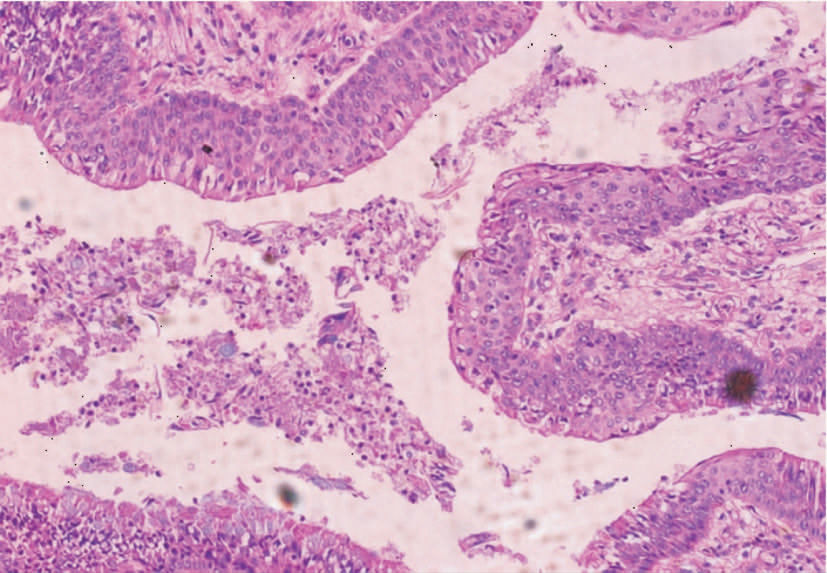
\includegraphics{./images/Image00110.jpg}
 \captionsetup{justification=centering}
 \caption{慢性支气管炎(HE染色,中倍)\\ {\small 支气管黏膜上皮变性、坏死,鳞状上皮化生}}
\label{fig7-1}
  \end{figure}

\paragraph{呼吸道腺体的病变}
为支气管炎的形态学特征。表现为黏膜上皮层内杯状细胞增多;黏液腺泡增生、肥大;浆液腺泡黏液化,黏液分泌增多。

\paragraph{管壁组织的损害}
急性发作时,黏膜层及黏膜下层充血、水肿,淋巴细胞、浆细胞及中性粒细胞浸润。炎症反复发作可破坏平滑肌、弹力纤维和软骨。支气管黏膜发生溃疡,管壁结缔组织增生,管腔狭窄,管腔内黏液栓潴留致气道阻塞。局部管壁塌陷、扭曲、变形。

\subsubsection{病理临床联系}

慢支患者缓慢起病,病程长,反复急性发作而病情加重。主要症状为咳嗽、咳痰,或伴有喘息。急性加重系指咳嗽、咳痰、喘息等症状突然加重,主要原因是呼吸道感染。由于黏液的分泌增多,痰液和炎症刺激支气管黏膜而引起咳嗽、咳痰。痰呈白色泡沫状,并发感染时可呈脓性。肺部听诊可闻及干湿性啰音。由于支气管黏膜肿胀、痰液阻塞和平滑肌痉挛,可出现哮喘样发作。

\subsubsection{并发症}

慢性支气管炎反复发作,病变逐渐加重。炎症向肺泡及支气管壁周围扩展,导致细支气管周围炎,还可发生纤维闭塞性支气管炎,以后引起阻塞性肺气肿、支气管扩张症,最终导致肺源性心脏病。长期炎症刺激可引起气管和支气管黏膜上皮发生鳞状上皮化生,进而发生不典型增生,最终恶变为鳞状细胞癌。

\subsection{支气管扩张症}

支气管扩张症(bronchiectasis)是由于支气管及其周围肺组织慢性化脓性炎症和纤维化,使支气管壁的肌肉和弹性组织破坏,导致支气管变形及持久扩张。典型的症状有慢性咳嗽、咳大量脓痰和反复咯血。主要致病因素为支气管感染、阻塞和牵拉,部分有先天遗传因素。患者多有麻疹、百日咳或支气管肺炎等病史。随着人民生活的改善,麻疹、百日咳疫苗的预防接种,以及抗生素的临床应用,本病的发病率大为减少。

\subsubsection{病因}

\paragraph{感染}
感染是引起支气管扩张的最常见原因。儿童时期麻疹、百日咳、流行性感冒(某些腺病毒感染)或严重的肺部感染如肺炎克雷白杆菌、葡萄球菌、流感病毒、真菌、分枝杆菌以及支原体感染,使支气管各层组织尤其是平滑肌纤维和弹性纤维遭到破坏,黏液纤毛清除功能降低,削弱了管壁的支撑作用,可继发支气管扩张。

\paragraph{支气管阻塞}
支气管由于受肿瘤、肿大淋巴结的压迫,或因腔内异物而发生不完全阻塞,使阻塞处以下的支气管腔内压力不断增大,管壁受损、管腔扩张。支气管完全阻塞时,其所属肺泡腔内空气被吸收而萎缩,该部位支气管壁受胸腔负压的牵拉而扩张。

\paragraph{先天性和遗传性疾病}
先天性较少见,是由于先天性支气管发育不良,存在先天性缺陷或遗传性疾病,使肺的外周不能进一步发育,导致已发育支气管扩张,如支气管软骨发育不全(Williams-Camplen综合征)。有的病人支气管扩张在出生后发生,但也有先天异常因素存在,如Kartagener综合征,患者除支气管扩张外可伴有内脏异位和胰腺囊性纤维化病变。支气管扩张症也可见于Young综合征,特征为阻塞性精子缺乏,慢性鼻窦炎,反复肺部感染和支气管扩张。部分支气管扩张病人显示免疫球蛋白缺陷,易于反复细菌感染。

\subsubsection{病理变化}

肉眼观:支气管扩张多发生于肺段及段以下支气管(Ⅲ~Ⅳ级支气管及细支气管)。常见于一个肺段,也可在双侧多个肺段发生。左肺较右肺多见,特别见于左肺下叶。扩张部支气管腔明显扩大,形态可分为圆柱状、囊状两种,亦常混合存在。柱状扩张者管壁破坏较轻,随着病变发展,破坏严重,乃出现囊状扩张(图\ref{fig7-2})。严重者肺组织呈蜂窝状。扩张的管腔内充满黄绿色黏稠脓性或血性渗出物。管壁黏膜萎缩或增生、肥厚,形成纵行皱襞。

\begin{figure}[!htbp]
 \centering
 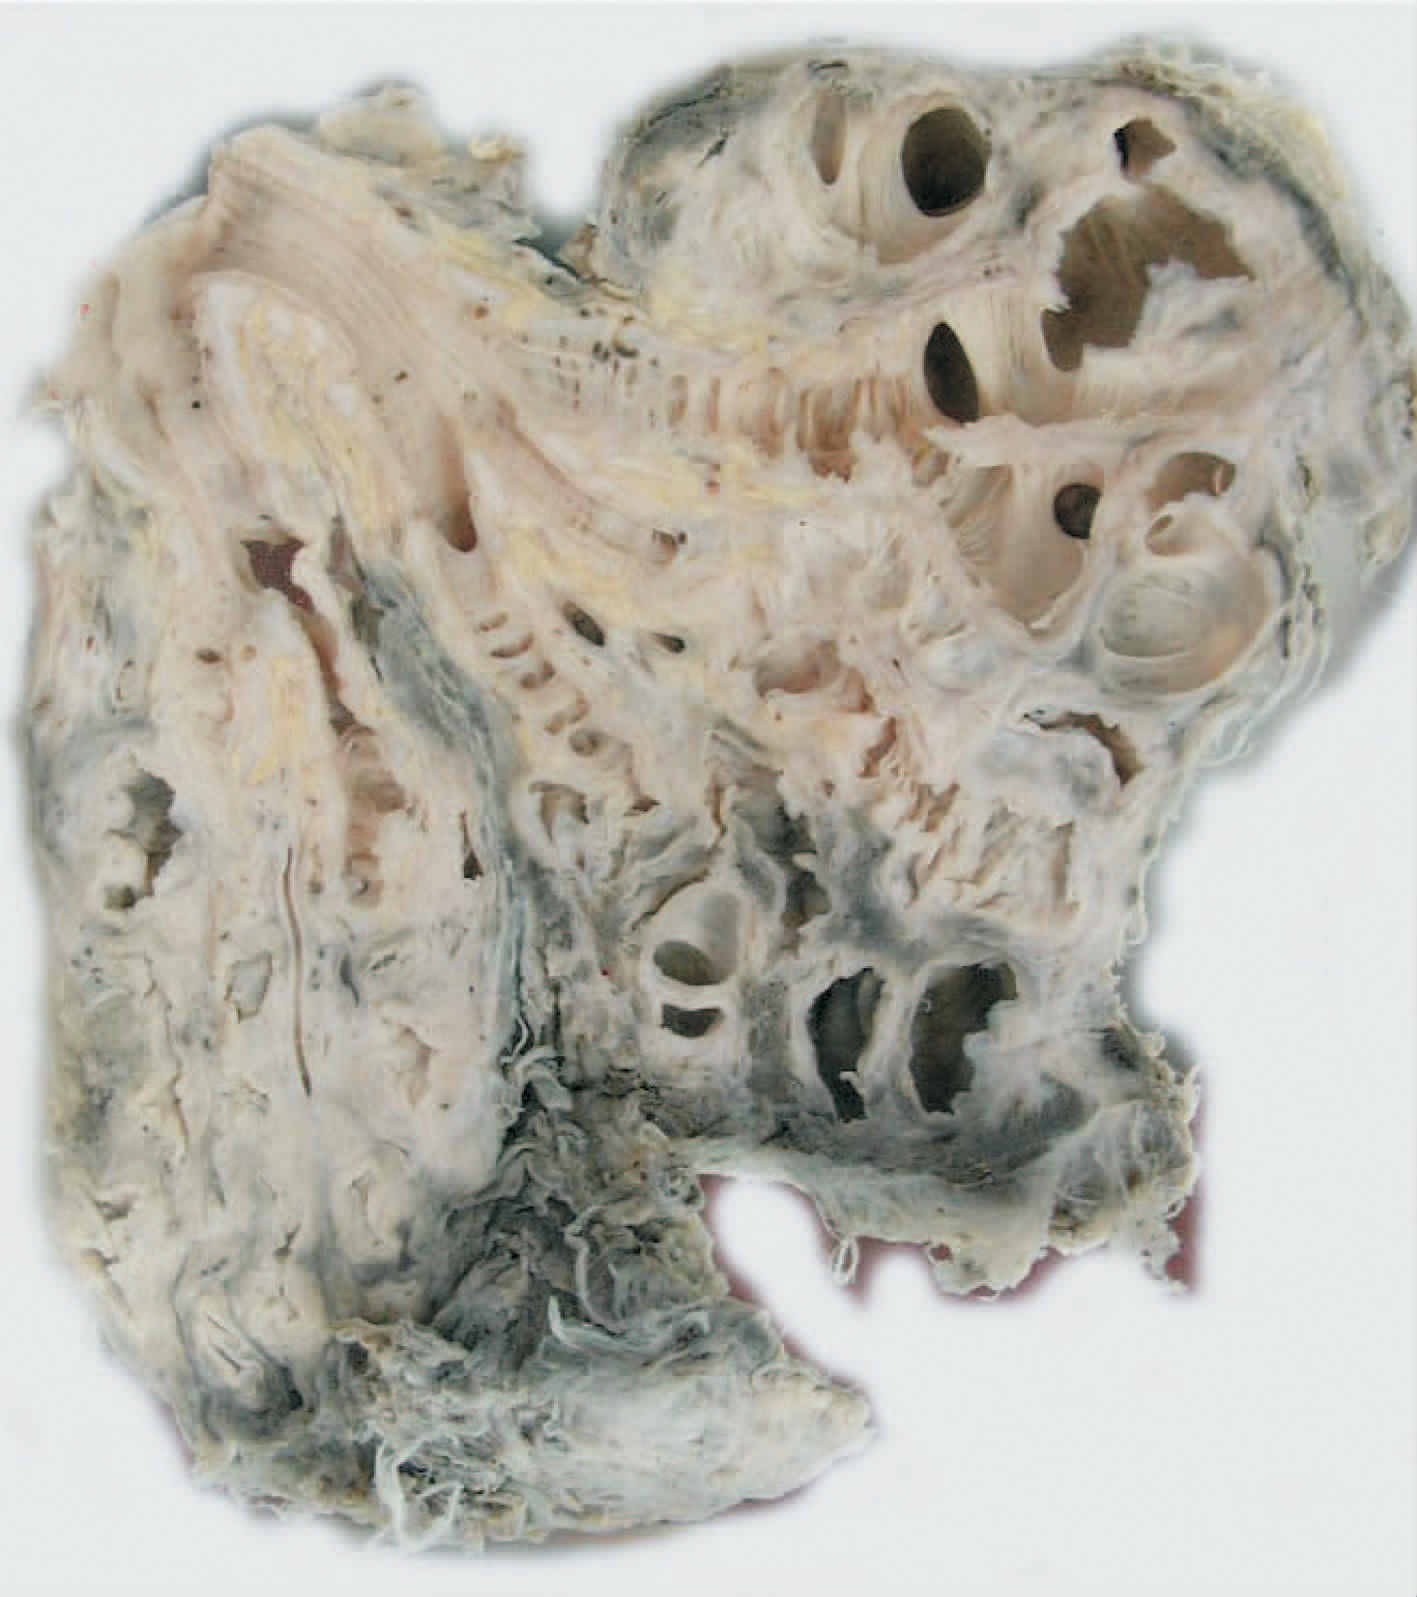
\includegraphics{./images/Image00111.jpg}
 \captionsetup{justification=centering}
 \caption{支气管扩张症\\ {\small 支气管呈圆柱状扩张,直达胸膜}}
\label{fig7-2}
  \end{figure}

镜下观:支气管呈慢性化脓性炎症,并伴有不同程度的组织破坏及管壁纤维化、瘢痕化。支气管扩张症易发生反复感染,其炎症可蔓延到邻近的肺实质,引起不同程度的肺炎、小脓肿或肺小叶不张以及慢性支气管炎的病变,久之可形成肺纤维化和阻塞性肺气肿,上述变化又加重支气管扩张。

\subsubsection{临床病理联系}

支气管扩张症的典型症状为慢性咳嗽、大量脓痰和反复咯血。咳嗽、咳痰主要是慢性炎症的刺激、黏液分泌增多及继发化脓菌感染所致。咳嗽和痰量与体位改变有关,尤其是清晨起床可咳出大量脓性痰,若有厌氧菌感染,则有臭味。咯血为小血管炎性破坏及咳嗽所致。有些患者仅表现为反复咯血,平时无咳嗽、脓痰等呼吸道症状,临床上称为“干性支气管扩张”。并发胸膜炎时,可出现胸痛。慢性重症支气管扩张症,肺组织广泛纤维化,病人可出现气急、发绀、杵状指(趾)。

\subsubsection{并发症}

支气管扩张症常见的并发症有肺脓肿、脓胸、脓气胸等。病灶内细菌经血道播散可到达远处器官,最常见的是引起脑膜炎、脑脓肿;由于抗菌药物的运用,此种情况已较少见。严重的支气管扩张致肺组织广泛纤维化,破坏肺血管床或形成支气管动脉与肺动脉分支吻合,则可导致肺动脉高压,引起肺心病。此外,在鳞状上皮化生的基础上可发生鳞状细胞癌。

\subsection{慢性阻塞性肺气肿}

慢性阻塞性肺气肿(chronic obstructive pulmonary
emphysema)是由于慢性支气管炎等引起呼吸性细支气管以远的末梢肺组织因残气量增多而呈持久性扩张,并伴有肺泡间隔破坏,以致肺组织弹性减弱,容积增大的阻塞性肺病。

\subsubsection{病因和发病机制}

肺气肿是支气管和肺疾病常见的并发症,与吸烟、空气污染、小气道感染、尘肺等关系密切,尤其是慢性阻塞性细支气管炎是引起肺气肿的重要原因。发病机制与下列因素有关:

\paragraph{阻塞性通气障碍}
慢性细支气管炎时,由于小气道的狭窄、阻塞或塌陷,导致阻塞性通气障碍,使肺泡内残气量增多。细支气管周围炎症使肺泡壁破坏、弹性减弱,末梢肺组织残气量不断增多而发生扩张,肺泡孔扩大,肺泡间隔断裂,扩张的肺泡互相融合形成气肿囊腔。此外,炎症损伤细小支气管壁软骨,细支气闭塞时,吸入的空气可经存在于细支气管和肺泡之间的Lambert孔进入闭塞远端的肺泡内(即肺泡侧流通气),而呼气时,Lambert孔闭合,空气不能排出,导致肺泡内储气量增多、肺泡内压增高。

\paragraph{弹性蛋白酶增多、活性增高}
与肺气肿发生有关的内源性蛋白酶主要是中性粒细胞和单核细胞释放的弹性蛋白酶。慢性支气管炎伴有肺感染尤其是吸烟者,肺组织内渗出的中性粒细胞和单核细胞较多,可释放多量弹性蛋白酶。此酶能降解肺组织中的弹性硬蛋白、结缔组织基质中的胶原和蛋白多糖,破坏肺泡壁结构。

\paragraph{遗传性α{1}-抗胰蛋白酶(α{1}-AT)缺乏}  α{1}
-抗胰蛋白酶由肝细胞产生,是一种分子量为45 000~56
000的糖蛋白,它能抑制蛋白酶、弹性蛋白酶、胶原酶等多种水解酶的活性。该酶缺失则增强了弹性蛋白酶的损伤作用。遗传性α{1}
-抗胰蛋白酶缺乏是引起原发性肺气肿的原因,α{1}
-抗胰蛋白酶缺乏的家族,肺气肿的发病率比一般人高15倍,主要是全小叶型肺气肿。

\subsubsection{病理变化}

\paragraph{肉眼观}
肺显著膨大,边缘钝圆,色泽灰白,表面常可见肋骨压痕,肺组织柔软而弹性差,指压后的压痕不易消退,触之捻发音增强。表面可见多个大小不一的大泡(图\ref{fig7-3})。

\begin{figure}[!htbp]
 \centering
 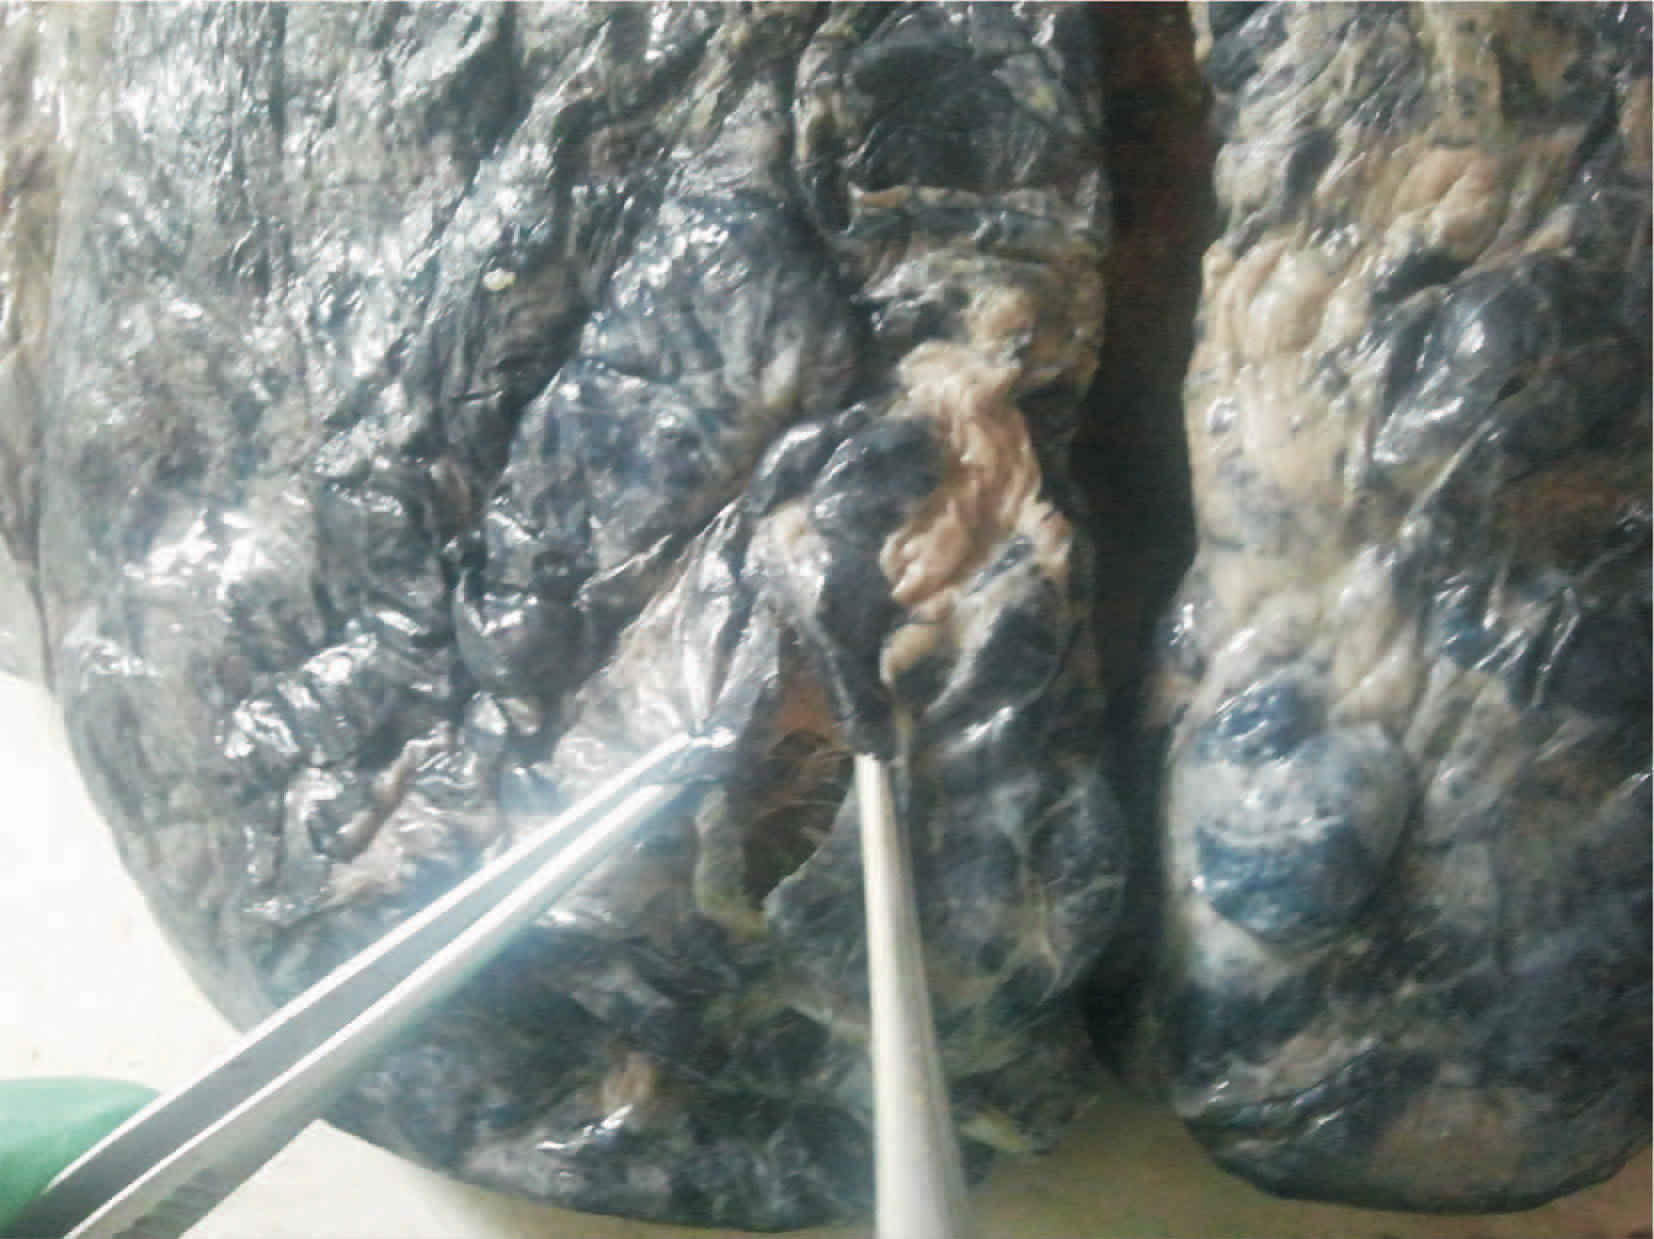
\includegraphics{./images/Image00112.jpg}
 \captionsetup{justification=centering}
 \caption{肺气肿}
 \label{fig7-3}
  \end{figure} 

\paragraph{镜下观}
肺泡扩张,间隔变窄,肺泡孔扩大,肺泡间隔断裂,扩张的肺泡融合成较大的囊腔。肺毛细血管床明显减少,肺小动脉内膜呈纤维性增厚。小支气管和细支气管可见慢性炎症。根据扩张部位又可分为小叶中央型、小叶周围型和全小叶型肺气肿(图\ref{fig7-4})。

(1)小叶中央型肺气肿:是临床最常见的一型。病变累及肺小叶的中央部分,呼吸性细支气管病变最明显,呈囊状扩张。而肺泡管、肺泡囊变化则不明显。

(2)全小叶型肺气肿:病变累及肺小叶的各个部位,从终末呼吸细支气管直至肺小叶和肺泡均呈弥漫性扩张,遍布于肺小叶内。如果肺泡间隔破坏较严重,气肿囊腔可融合成直径超过1
cm的大囊泡,形成大泡性肺气肿。

(3)小叶周围型肺气肿:病变主要累及肺小叶远端部位的肺泡囊,而近端部位的呼吸性细支气管和肺泡管基本正常。常合并有小叶中央型和全小叶型肺气肿。

肺气肿的气肿囊泡为扩张的呼吸性细支气管,在近端囊壁上常可见呼吸上皮(柱状或低柱状上皮)及平滑肌束的残迹。全小叶型肺气肿的气肿囊泡主要是扩张变圆的肺泡管和肺泡囊,有时还可见到囊泡壁上残留的平滑肌束片断,在较大的气肿囊腔内有时还可见含有小血管的悬梁。

\begin{figure}[!htbp]
 \centering
 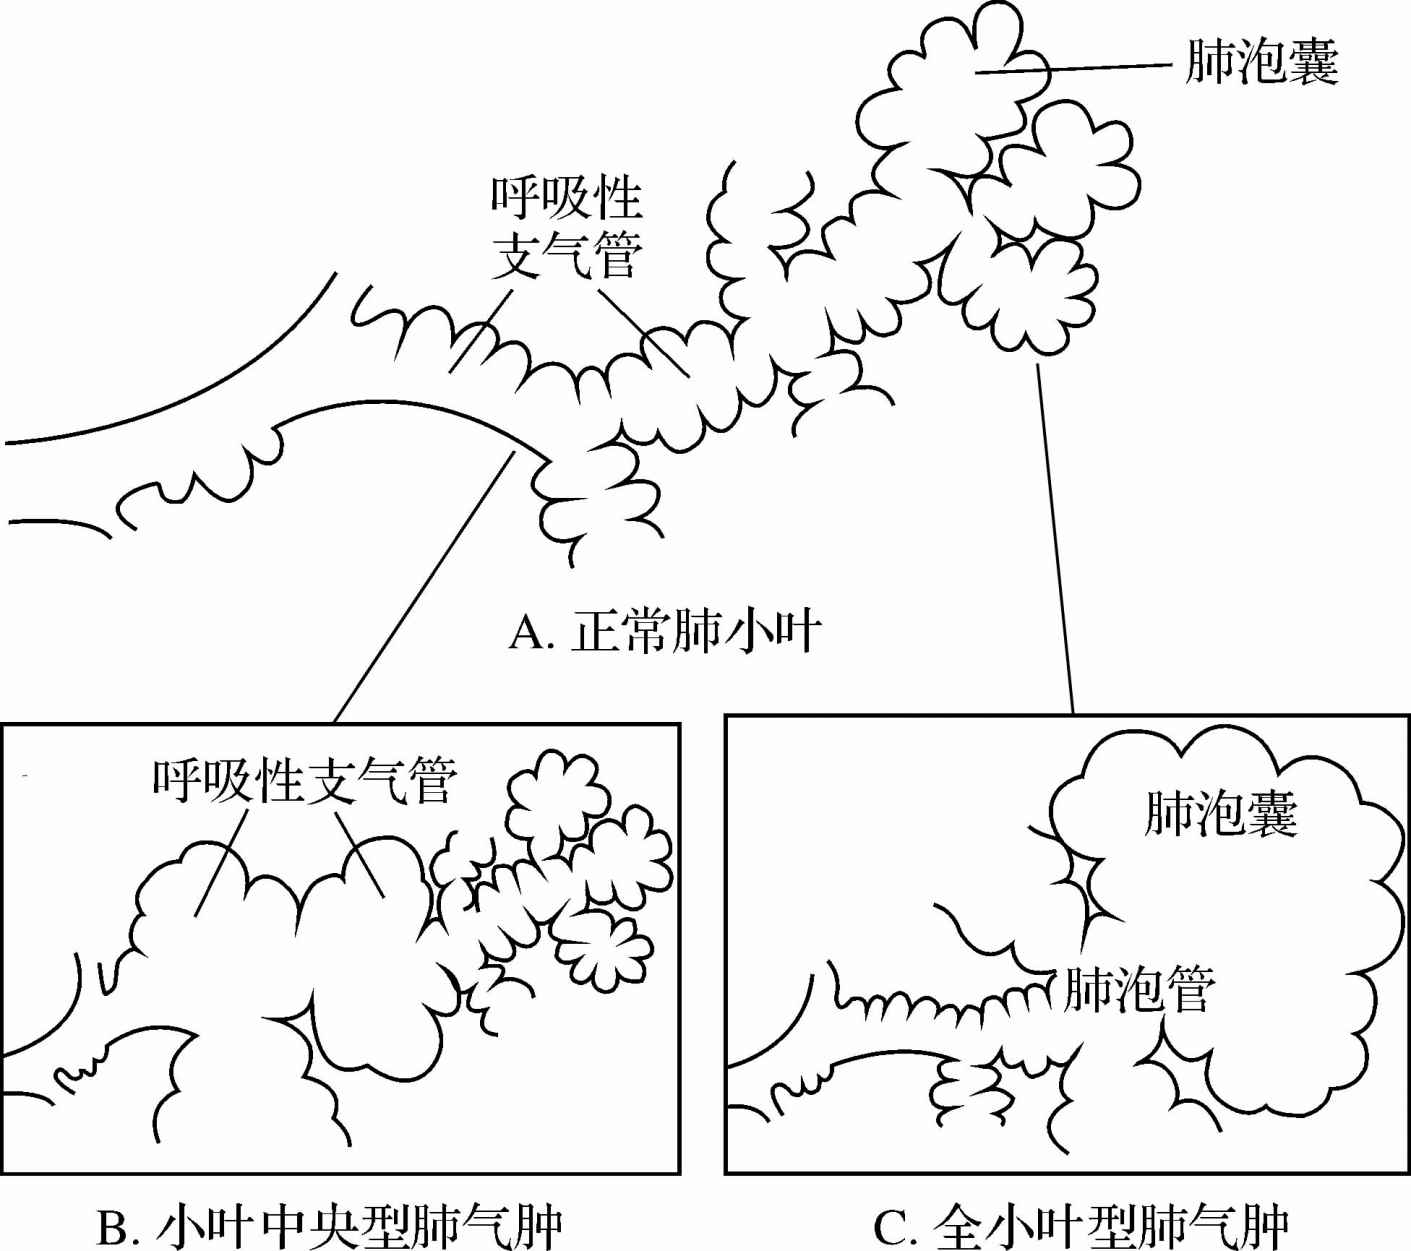
\includegraphics{./images/Image00113.jpg}
 \captionsetup{justification=centering}
 \caption{慢性阻塞性肺气肿类型模式图}
 \label{fig7-4}
  \end{figure} 

\subsubsection{临床病理联系及转归}

肺气肿患者的主要症状是气短,轻者仅在体力劳动时发生,随着气肿程度加重,气短逐渐明显,甚至休息时也出现呼吸困难,并常感胸闷。每当合并呼吸道感染时,症状加重,并可出现缺氧、酸中毒等一系列症状。患者胸廓前后径增大,呈桶状胸。胸廓呼吸运动减弱。叩诊呈过清音,心浊音界缩小或消失,肝浊音界下降。语音震颤减弱。听诊时呼吸音减弱,呼气延长,用力呼吸时两肺底部可闻及湿啰音和散在的干啰音。剑突下心音增强,肺动脉瓣第二音亢进。

肺气肿严重时可引起肺源性心脏病及衰竭。肺大泡破裂后引起自发性气胸,并可导致大面积肺萎陷。由于外呼吸功能严重障碍,导致呼吸衰竭及肺性脑病。呼吸衰竭时发生的低氧血症和高碳酸血症会引起各系统的代谢功能严重紊乱。中枢神经系统对缺氧最为敏感,随着缺氧程度的加重,可出现一系列中枢神经系统功能障碍,由开始的大脑皮层兴奋性增高而后转入抑制状态。病人表现由烦躁不安、视力和智力的轻度减退,逐渐发展为定向和记忆障碍,精神错乱、嗜睡、惊厥以至意识丧失。

\section{肺源性心脏病}

肺源性心脏病(cor
pulmonale,)简称肺心病,主要由于支气管肺组织、胸廓或肺动脉血管病变所致肺循环阻力增加,肺动脉高压,导致右心室肥厚、扩张而引起的心脏病。根据起病缓急和病程长短,可分为急性和慢性两类。临床上后者多见,除原有肺、胸疾病的各种症状和体征外,主要是逐步出现肺、心功能衰竭以及其他器官损害的征象。

\subsection{病因}

\paragraph{支气管、肺疾病}
以慢支并发阻塞性肺气肿最为多见,占80%~90%,其次为支气管哮喘、支气管扩张、重症肺结核、尘肺、慢性弥漫性肺间质纤维化、结节病、过敏性肺泡炎、嗜酸性肉芽肿等。

\paragraph{胸廓运动障碍性疾病}
较少见,严重的脊椎后、侧凸,脊椎结核,类风湿关节炎,胸膜广泛粘连及胸廓形成术后造成的严重胸廓或脊椎畸形,以及神经肌肉疾患如脊髓灰质炎,可引起胸廓活动受限、肺受压、支气管扭曲或变形,导致肺功能受限,气道引流不畅,肺部反复感染,并发肺气肿,或纤维化、缺氧、肺血管收缩、狭窄,使阻力增加,肺动脉高压,发展成肺心病。

\paragraph{肺血管疾病}
甚少见。累及肺动脉的过敏性肉芽肿病,广泛或反复发生的多发性肺小动脉栓塞及肺小动脉炎,以及原因不明的原发性肺动脉高压症,均可使肺小动脉狭窄、阻塞,引起肺动脉血管阻力增加、肺动脉高压和右心室负荷加重,发展成肺心病。

\subsection{发病机制}

上述任何因素引起肺心病的关键环节都是肺动脉高压,其发病机制如下:

\paragraph{肺毛细血管床显著减少}
慢性肺气肿或肺广泛纤维化,使肺泡壁毛细血管受压、扭曲变形,甚至管腔狭窄或闭锁,肺毛细血管床总横断面积减少,从而肺循环阻力增加,肺动脉压升高。

\paragraph{肺内血管分流}
在慢性肺部疾病时,肺泡壁毛细血管受压闭塞,或因肺组织广泛纤维化,肺循环的正常途径受阻,使肺动脉和支气管动脉之间的吻合支开放,压力高的支气管动脉血流入压力低的肺动脉系统,引起肺动脉压升高。

\paragraph{肺通气、换气功能障碍}
严重的慢性肺部疾病可引起肺通气、换气功能障碍,导致缺氧、高碳酸血症和呼吸性酸中毒,使小动脉痉挛收缩,并刺激血管平滑肌细胞,使之增生、肥大,血管壁增厚,引起肺循环阻力增大,肺动脉压升高。慢性缺氧还可产生继发性红细胞增多、血液黏稠度增加,血流阻力随之增高。缺氧还引起肾动脉收缩,肾血流量减少,醛固酮分泌增加,从而引起水、钠潴留,血容量增多,更使肺动脉压升高。临床上缺氧和高碳酸血症得到纠正后,肺动脉压可明显降低,部分病人甚至可恢复到正常范围。

\subsection{病理变化}

肺心病是多种慢性肺部疾病的晚期并发症,形成肺血管改变和右心室肥厚扩张。因此,肺心病的病理变化包括晚期肺部疾病、肺血管和心脏三种病变。肺部疾病详见有关章节,此处仅叙述肺血管和心脏病变。

\subsubsection{肺血管病变}

肺小动脉及其分支的病变在肺动脉高压的形成中起着重要作用,表现为:①肺小动脉中膜平滑肌增生肥大,细胞外基质合成增多,致肺小动脉中膜肥厚,使肺小动脉管壁增厚、变硬,管腔狭窄,肺循环阻力增加。②无肌细动脉肌化:持续缺氧可以刺激肺泡毛细血管前的无肌细动脉管壁平滑肌增生。③肺小、细动脉内膜下胶原纤维增生,并出现纵行肌束。上述改变使肺小、细动脉管壁增厚,管腔狭窄(图\ref{fig7-5})。④肺小动脉炎:若肺部炎症累及邻近的肺小动脉,引起血管的急、慢性炎,致使病变处血管管壁增厚、管腔狭窄或纤维化。⑤肺泡壁毛细血管床数量显著减少。

\begin{figure}[!htbp]
 \centering
 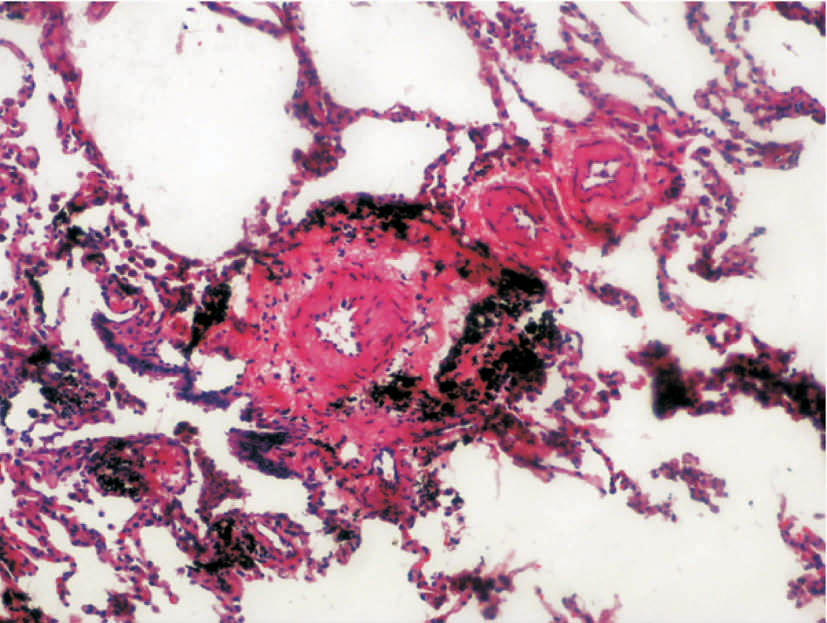
\includegraphics{./images/Image00114.jpg}
 \captionsetup{justification=centering}
 \caption{慢性肺源性心脏病肺小动脉硬化\\ {\small 镜下见肺细动脉管壁增厚,管腔狭窄(HE染色,中倍)}}
\label{fig7-5}
  \end{figure}

\subsubsection{心脏病变}

肉眼观:心脏体积明显增大,重量增加,平均为326 g,最重者可达785
g。右心室壁显著肥厚,后期心腔扩张。心尖钝圆,肺动脉圆锥隆起(图\ref{fig7-6}A),肺动脉瓣下2
cm处右心室肌壁厚度超过0.5 cm。

镜下观:右心室心肌纤维肥大(图\ref{fig7-6}B),可见肌浆溶解、变性、坏死,间质水肿和结缔组织增生。

\begin{figure}[!htbp]
 \centering
 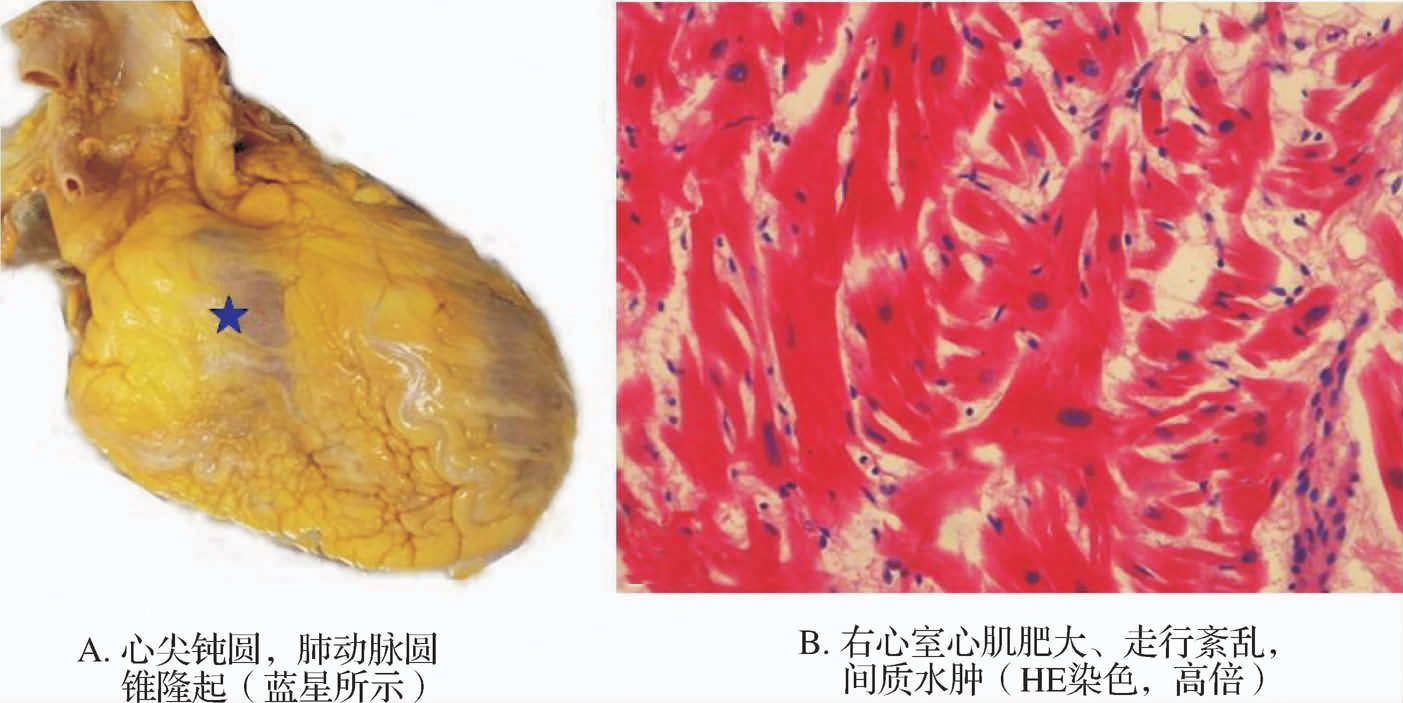
\includegraphics{./images/Image00115.jpg}
 \captionsetup{justification=centering}
 \caption{慢性肺源性心脏病}
 \label{fig7-6}
  \end{figure} 

\subsection{临床病理联系}

肺心病进展缓慢,开始主要表现为原来肺部疾病的症状。随着病变加重,肺动脉压升高,右心负荷增加,患者出现心慌、气急、发绀及下肢水肿、肝肿大等右心力衰竭的症状和体征。重症肺心病,由于呼吸功能衰竭所致缺氧、二氧化碳潴留可引起肺性脑病,患者表现为头痛、烦躁、精神错乱、意识不清和昏迷等,是肺心病患者重要致死原因。

\section{肺炎}

肺炎(pneumonia)通常是指肺的急性渗出性炎症,为呼吸系统的多发病、常见病。在我国各种致死病因中,肺炎占第5位。肺炎按病因可分为感染性肺炎,如细菌性肺炎、病毒性肺炎、支原体肺炎、真菌性肺炎及其他病原体包括立克次体、肺炎衣原体、寄生虫(如弓形体、卡氏肺孢子虫、肺包虫、肺吸虫)等引起的肺炎等。理化因素引起的肺炎,如放射性、吸入性、类脂性肺炎以及变态反应性(如过敏性和风湿性)肺炎等。由于致病因子和机体反应性的不同,炎症发生的部位、累及范围和病变性质也往往不同。炎症发生于肺泡内者称肺泡性肺炎(大多数肺炎为肺泡性),累及肺间质者称间质性肺炎。病变范围以肺小叶为单位者称小叶性肺炎,累及肺段者称节段性肺炎,波及整个或多个大叶者称大叶性肺炎。按病变性质可分为浆液性、纤维素性、化脓性、出血性、干酪性、肉芽肿性或机化性肺炎等不同类型。

\subsection{大叶性肺炎}

大叶性肺炎(lobar
pneumonia)主要是由肺炎链球菌感染引起的肺组织的急性纤维素性渗出性炎症。病变起始于肺泡,并迅速扩展至整个或多个大叶。多见于青壮年,好发于冬、春季节。临床表现为骤然起病、寒战高热、胸痛、咳嗽、咳铁锈色痰、呼吸困难,并有肺实变体征及白细胞增高等。典型病程7~10天。

\subsubsection{病因和发病机制}

95%以上的大叶性肺炎由肺炎链球菌引起,尤以Ⅲ型者毒力最强。此外,肺炎杆菌、金黄色葡萄球菌、溶血性链球菌、流感嗜血杆菌也可引起。本病主要经呼吸道感染,受寒、疲劳、醉酒、感冒、麻醉、糖尿病、肝肾疾病等均为其诱因。此时,呼吸道防御功能被削弱,机体抵抗力降低,易发生细菌感染。细菌侵入肺泡后在其中繁殖,引起肺泡壁水肿,继而白细胞渗出和红细胞漏出,特别是形成的浆液性渗出物有利于细菌繁殖,并使细菌通过肺泡间孔(Cohn孔)或呼吸性细支气管迅速向邻近肺组织蔓延,从而波及肺段或整个大叶。在肺大叶之间的蔓延则系带菌渗出液经叶支气管播散所致。

\subsubsection{病理变化及与临床联系}

病变一般多见于左肺下叶,也可同时或先后发生于两个以上肺叶。由于毛细血管通透性增高,大量纤维蛋白原渗出于肺泡,使肺组织大面积广泛实变。按自然病程可分为四期。

\paragraph{充血水肿期}
发病后1~2天,肺叶充血、水肿,暗红色,切开时有血性浆液自切面流出。镜下观:肺泡壁毛细血管扩张充血,肺泡腔内有大量浆液性渗出物,混有少数红细胞、中性粒细胞和巨噬细胞,并含有大量细菌(图\ref{fig7-7})。

临床上出现高热、寒战、白细胞增多等毒血症症状,听诊可闻及湿性啰音,X线检查病变处呈现淡薄、均匀的阴影,渗出物中可检出大量肺炎双球菌。

\begin{figure}[!htbp]
 \centering
 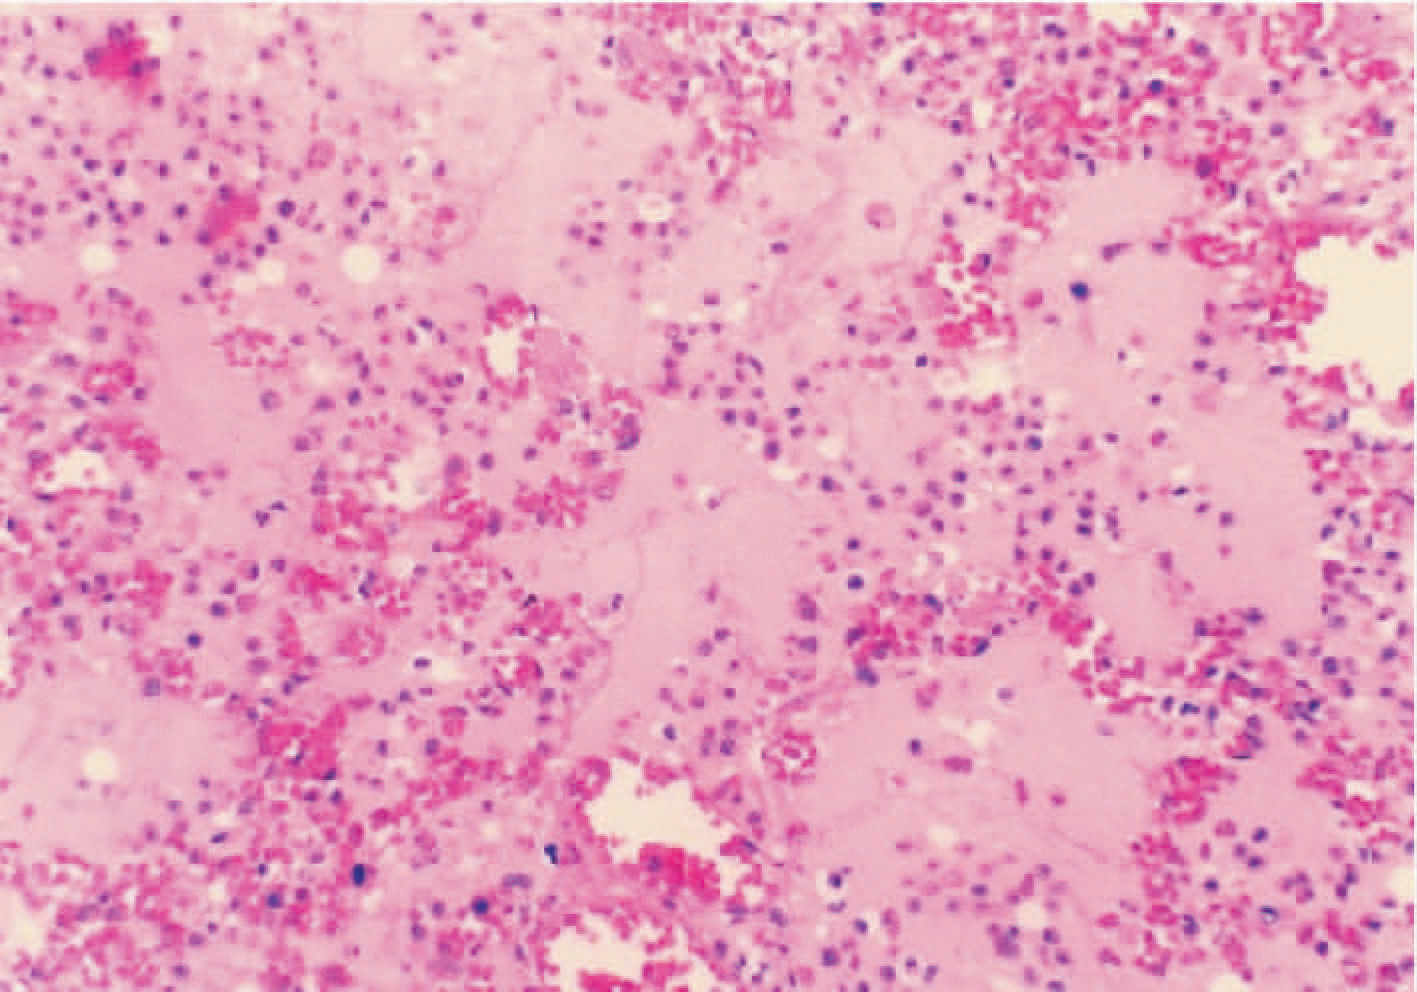
\includegraphics{./images/Image00116.jpg}
 \captionsetup{justification=centering}
 \caption{大叶性肺炎(充血水肿期)(HE染色,中倍)\\ {\small 肺泡壁毛细血管高度充血水肿,肺泡腔内充满浆液,其中混有少量红细胞和白细胞}}
\label{fig7-7}
  \end{figure}

\paragraph{红色肝样变期}
1~2天后,即有大量纤维蛋白原渗出。肉眼观:肺叶肿大,颜色暗红,质实如肝,切面颗粒状,为充塞于肺泡腔内的纤维素性渗出物突出于切面所致。病变肺叶的胸膜面常有纤维素性渗出物覆盖。镜下观:肺泡壁毛细血管显著充血,肺泡腔内充满混有红细胞、中性粒细胞、巨噬细胞的纤维素性渗出物,纤维素可穿过肺泡间孔与相邻肺泡中的纤维素相互连接成网状,有利于中性粒细胞和巨噬细胞的吞噬作用,防止细菌扩散(图\ref{fig7-8})。

\begin{figure}[!htbp]
 \centering
 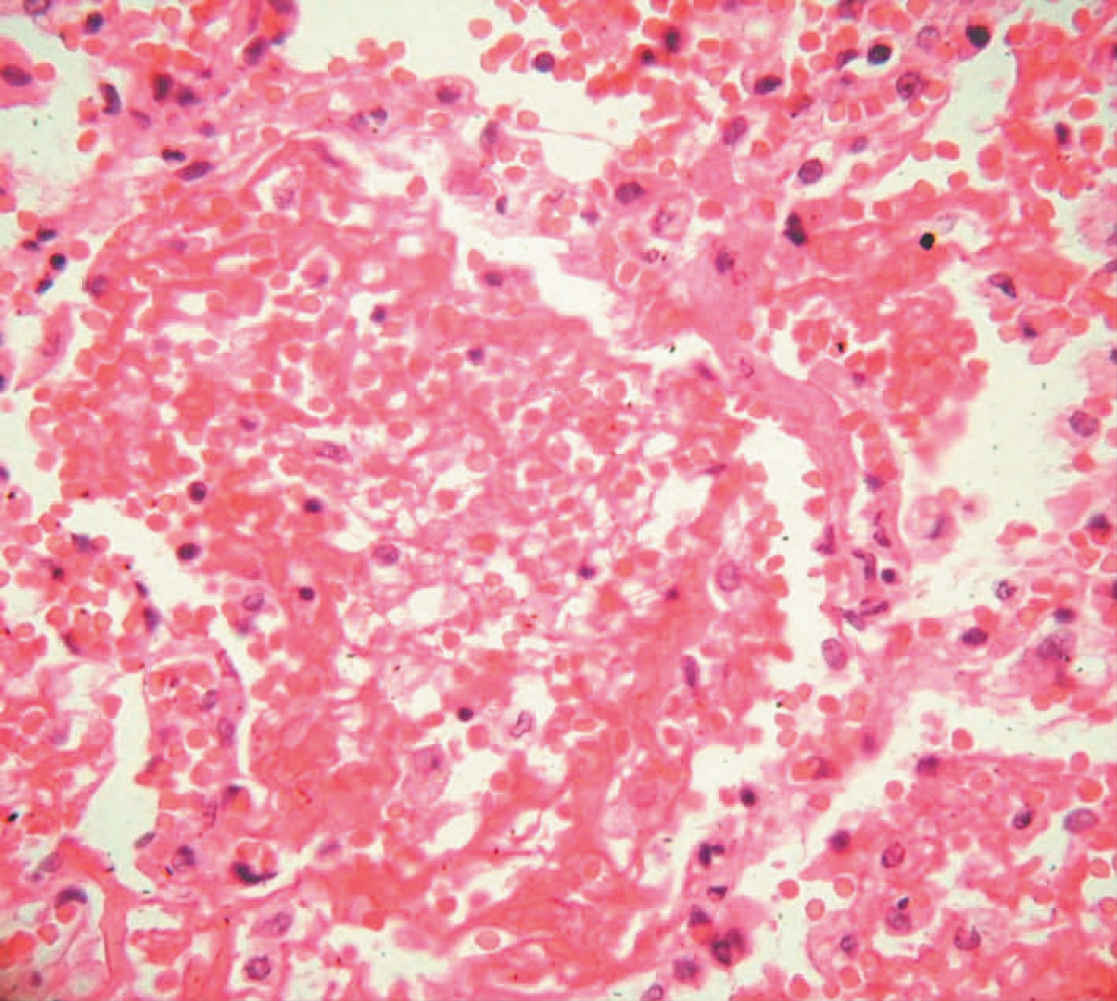
\includegraphics{./images/Image00117.jpg}
 \captionsetup{justification=centering}
 \caption{大叶性肺炎红色肝样变期(HE染色,高倍)\\ {\small 肺泡壁毛细血管高度扩张、充血,肺泡腔中含大量纤维素、红细胞及少量白细胞}}
\label{fig7-8}
  \end{figure}

临床上,病人高热稽留不退,呼吸急促。由于红细胞破坏与崩解,被巨噬细胞吞噬,形成含铁血黄素,经痰液排出,使痰呈铁锈色。由于病变累及胸膜,病人常感胸痛。若病变范围较大,实变区的大量静脉血未能氧合便流入左心,引起血氧分压和氧饱和度降低,病人可出现发绀、呼吸困难等缺氧表现。胸部叩诊呈浊音,听诊闻及管性呼吸音和胸膜摩擦音,X线检查见大片致密阴影。渗出物中仍可检出肺炎双球菌。

\paragraph{灰色肝样变期}
在发病4~6天后,肺泡腔内纤维素性渗出物及中性粒细胞继续增加。肉眼观:病变肺叶质实如肝,明显肿胀,重量增加,呈灰白色。如血管损伤较重、出血较多,外观可呈红色。胸膜面仍有纤维素性渗出物覆盖。镜下观:肺泡腔内充满大量纤维素及中性粒细胞,红细胞大部分破坏溶解,被咳出或被吸收。由于肺泡腔内渗出物的压力,肺泡壁毛细血管受压而处于贫血状态(图\ref{fig7-9})。

\begin{figure}[!htbp]
 \centering
 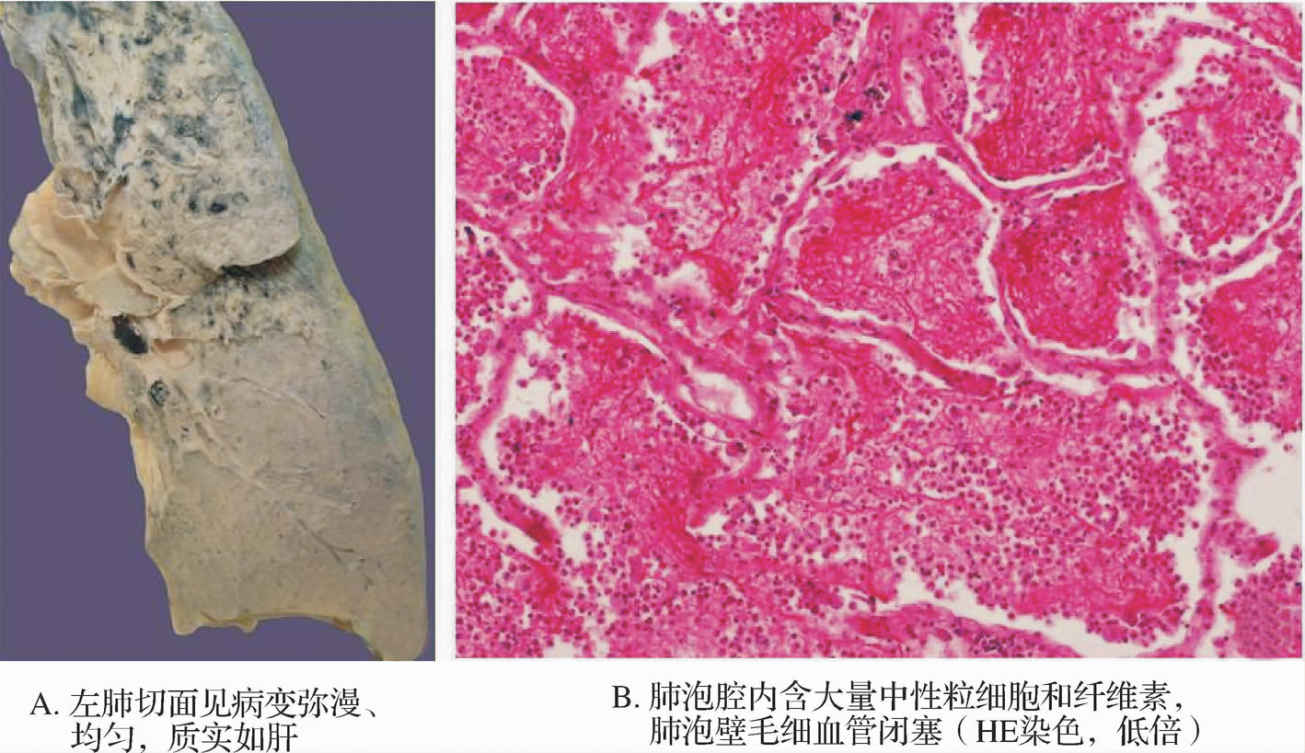
\includegraphics{./images/Image00118.jpg}
 \captionsetup{justification=centering}
 \caption{大叶性肺炎灰色肝样变期}
 \label{fig7-9}
  \end{figure} 

临床上,痰呈脓性,因肺泡壁毛细血管受压,流经病变区的血流量减少,肺静脉血氧合不足的情况反而减轻,故缺氧状况有所改善。听诊及X线检查所见与红色肝样变期表现基本相同。由于特异性抗体的产生或吞噬作用的加强,此期肺炎双球菌大多已被消灭,故不易检出。

\paragraph{溶解消散期}
经5~10天,炎症消退。肉眼观:肺叶质地变软,色转灰红,切面颗粒状外观消失。细菌被吞噬细胞吞噬清除,渗出物被溶解,或经淋巴管吸收或被咳出。肺泡腔逐渐排空,重新充气。大叶性肺炎时,肺组织常无坏死,肺泡壁结构也未遭破坏,愈复后,肺组织可完全恢复其正常结构和功能。胸膜渗出物可完全吸收,否则可遗留胸膜增厚或粘连(图\ref{fig7-10})。

临床上病人体温下降,症状消退,由于渗出物的液化排出,肺部又可闻及湿性啰音。X线检查见病变处阴影密度减低,透亮度逐渐增加。2~3周后肺实变体征完全消失。

大叶性肺炎的一个重要特点是在整个病程中,肺泡壁结构通常未遭破坏,愈合后肺组织可完全恢复正常结构和功能。支气管的炎症病变轻微,仅有充血、点状出血和小支气管黏膜上皮脱落等,晚期可完全恢复正常。

\begin{figure}[!htbp]
 \centering
 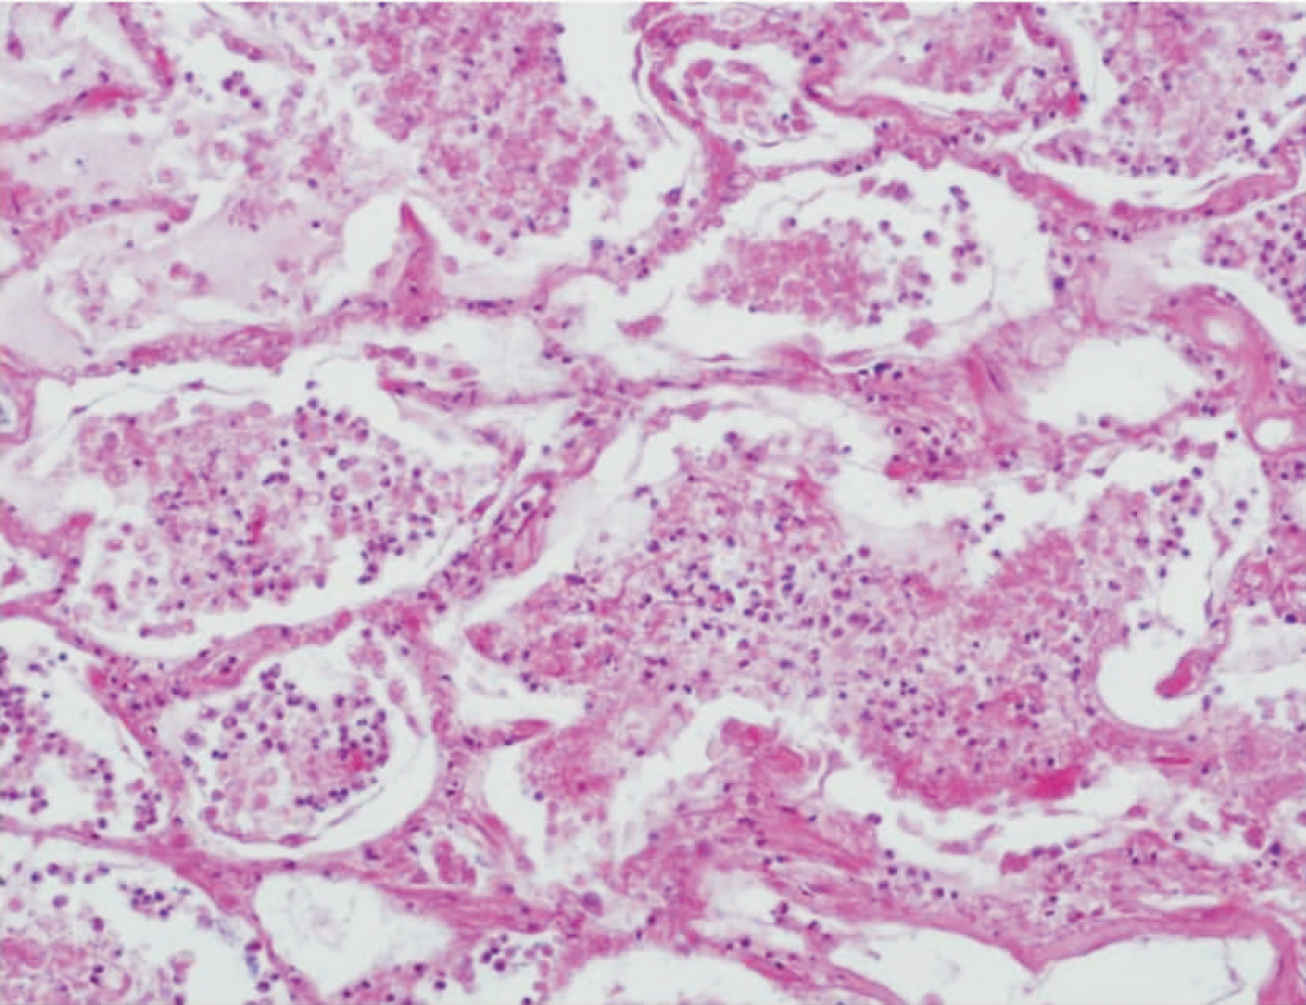
\includegraphics{./images/Image00119.jpg}
 \captionsetup{justification=centering}
 \caption{大叶性肺炎消散期\\ {\small 肺泡腔内的渗出物逐渐溶解、吸收,肺泡壁部分毛细血管重新开放(HE染色,低倍)}}
\label{fig7-10}
  \end{figure}

\subsubsection{结局和并发症}

不伴有并发症的大叶性肺炎经过一般治疗,病人在发病后7~10天,体温下降,症状好转,趋向痊愈。需要指出的是,病变的发展是一个连续过程,因而上述分期不是绝对的,特别是抗生素广泛用于临床以来,上述典型病程已很少见到。抗生素的及时应用能减轻病情、缩短病程、提早康复。少数病例可出现以下并发症:

\paragraph{感染性休克}
是最严重的并发症。病人出现高热,血压下降,四肢厥冷,多汗,口唇青紫等休克症状,称休克型或中毒型肺炎。如果抢救不及时,病死率较高。

\paragraph{肺肉质变}
少数病例肺泡腔内渗出物未被及时溶解、清除,由肺泡壁增生的肉芽组织替代,发生机化,使局部肺组织形成肉样组织,称肺肉质变。

\paragraph{败血症}
严重感染时,细菌侵入血液繁殖,形成败血症,可引起心内膜炎、脑膜炎及关节炎等。

\paragraph{肺脓肿、脓胸}
由于抗生素的早期应用,临床已少见。

\subsection{小叶性肺炎}

小叶性肺炎(lobular
pneumonia)主要由化脓菌感染引起,病变起始于细支气管,并以细支气管为中心、向周围或末梢肺组织发展,形成以肺小叶为单位、呈灶状散布的肺化脓性炎。因其病变以支气管为中心故又称支气管肺炎(bronchopneumonia)。主要发生于小儿、年老体弱者或久病卧床者,冬、春季节发病率增高。

\subsubsection{病因和发病机制}

小叶性肺炎主要由细菌感染引起,最常见的细菌为致病力较弱的肺炎球菌,其次为葡萄球菌、链球菌、肺炎球菌、流感嗜血杆菌、铜绿假单胞菌和大肠埃希菌等。这些细菌通常是口腔或上呼吸道内致病力较弱的常驻寄生菌,往往在某些诱因影响下,如患传染病、营养不良、恶病质、慢性心力衰竭、昏迷、麻醉、手术后等,使机体抵抗力下降,呼吸系统的防御功能受损,细菌得以入侵、繁殖,发挥致病作用,引起支气管肺炎。因此,支气管肺炎常是某些疾病的并发症,如麻疹后肺炎、手术后肺炎、吸入性肺炎、坠积性肺炎等。有时成为病人的直接死亡原因,故又有临终性肺炎之称。

\subsubsection{病理变化}

以细支气管为中心的肺组织化脓性炎是小叶性肺炎的特征。

肉眼观:肺组织内散布一些以细支气管为中心的化脓性炎症病灶,常散布于两肺各叶,尤以背侧和下叶病灶较多。病灶大小不等,直径多在1
cm左右(相当于肺小叶范围),形状不规则,色暗红或带黄色(图\ref{fig7-11}A)。严重者,病灶互相融合甚或累及全叶,形成融合性支气管肺炎。

镜下观:病灶中支气管、细支气管及其周围的肺泡腔内充满脓性渗出物,纤维蛋白一般较少(图\ref{fig7-11}B)。病灶周围肺组织充血,可有浆液渗出、肺泡过度扩张等变化。由于病变发展阶段的不同,各病灶的病变表现和严重程度亦不一致。有些病灶完全化脓,支气管和肺组织遭破坏,而另一些病灶内则仅可见浆液性渗出,有的还停留于细支气管及其周围炎阶段。

\begin{figure}[!htbp]
 \centering
 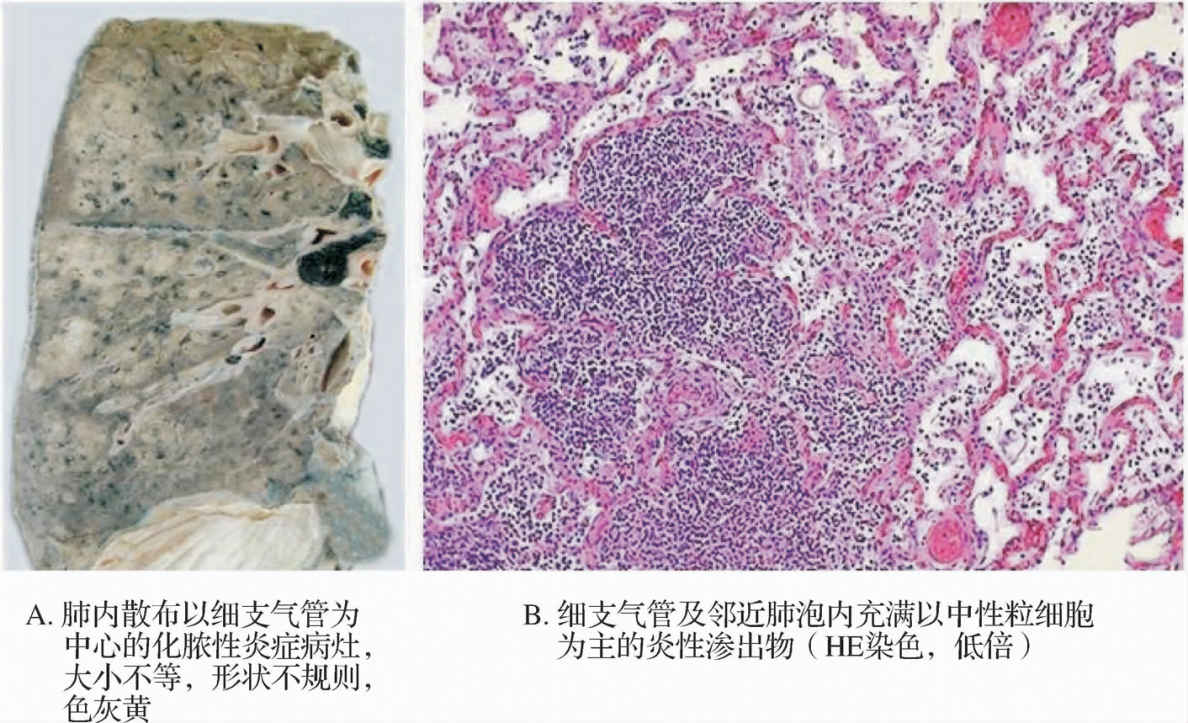
\includegraphics{./images/Image00120.jpg}
 \captionsetup{justification=centering}
 \caption{小叶性肺炎}
 \label{fig7-11}
  \end{figure} 

\subsubsection{临床病理联系}

因小叶性肺炎多为其他疾病的并发症,其临床症状常为原发性疾病所掩盖。由于支气管黏膜的炎症刺激而引起咳嗽,痰呈黏液脓性。因病变常呈灶性散布,肺实变体征一般不明显。病变区细支气管和肺泡内含有渗出物,听诊可闻湿啰音。X线检查可见肺野内散在不规则小片状或斑点状模糊阴影。

\subsubsection{结局和并发症}

小叶性肺炎若治疗及时,多数病例预后良好。如病人为年老、体弱、婴幼儿或作为其他疾病的并发症,则预后较差。常见的并发症有肺脓肿、脓胸、支气管扩张症。严重的小叶性肺炎,病变范围广泛者可并发呼吸功能及心功能不全。

\subsection{间质性肺炎}

间质性肺炎(interstitial
pneumonia)指发生于肺间质的炎症,以淋巴细胞、巨噬细胞浸润为特征。肺间质包括肺泡壁、肺小叶间隔及细支气管周围组织。间质性肺炎的病变及临床症状与大叶性肺炎、小叶性肺炎均不相同,主要由肺炎支原体和病毒引起,其肺部的病理变化大致相似。

其基本病理变化为:

肉眼观:病变常位于一侧肺叶,偶有累及两肺者,以肺下叶较多见。病灶多呈斑片状,红黄色。镜下观:肺泡壁增厚,充血,水肿,常有多量淋巴细胞、巨噬细胞浸润,偶见浆细胞。肺泡腔内渗出物不明显,仅见少量浆液及少数巨噬细胞(图\ref{fig7-12})。

\begin{figure}[!htbp]
 \centering
 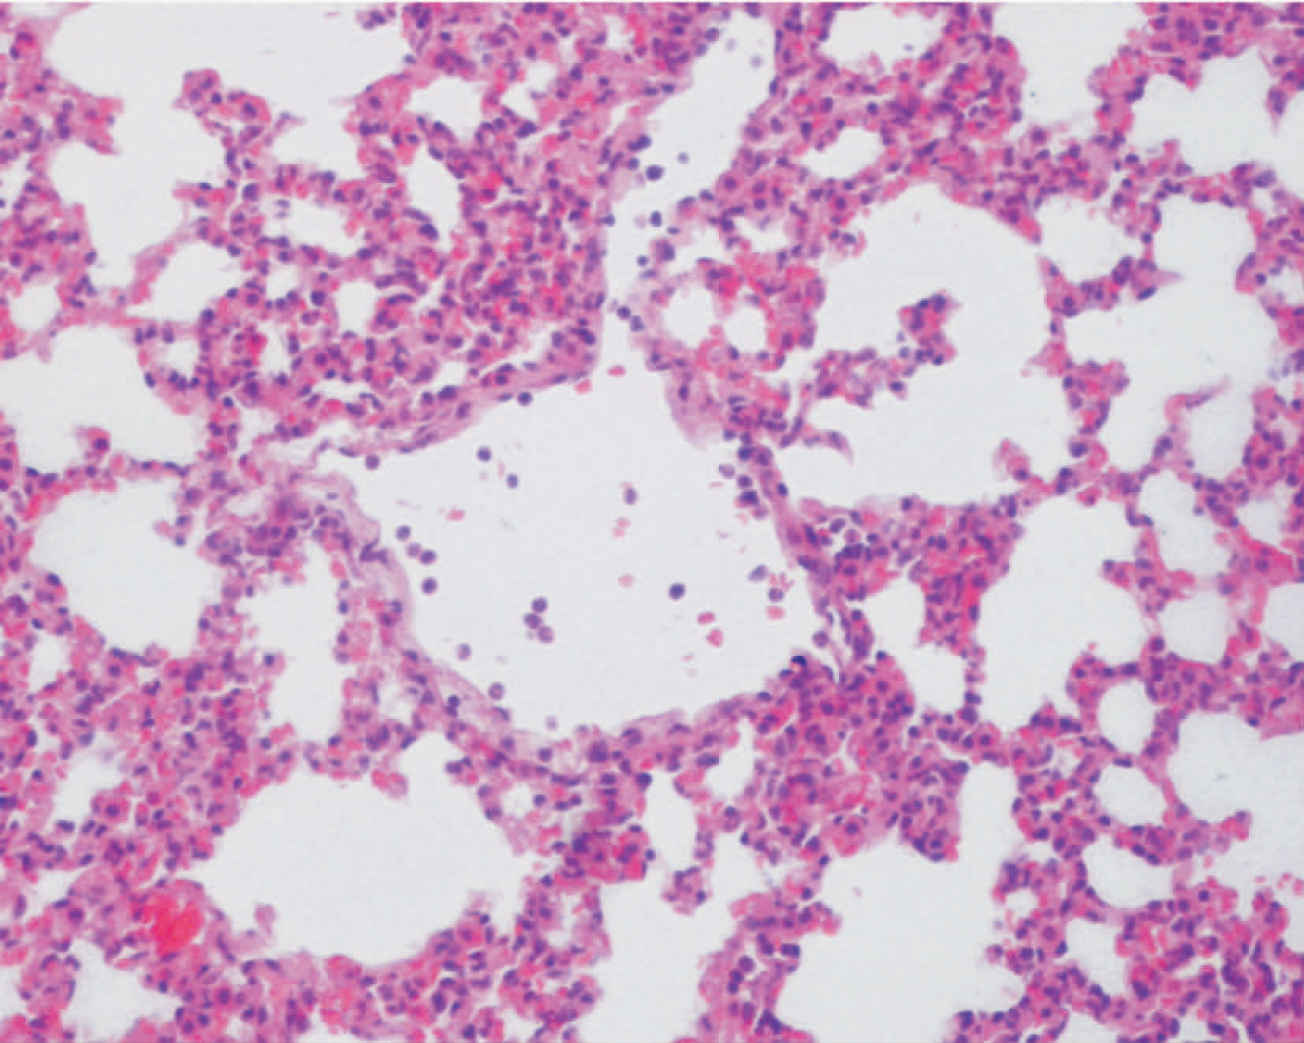
\includegraphics{./images/Image00121.jpg}
 \captionsetup{justification=centering}
 \caption{间质性肺炎(HE染色,中倍)\\ {\small 肺间质内有多量巨噬细胞和淋巴细胞浸润,肺泡腔内渗出物少}}
\label{fig7-12}
  \end{figure}

因病原不同,本病病变又各具特点,现分述如下:

\subsubsection{支原体肺炎}

支原体肺炎(mycoplasmal
pneumonia)是由肺炎支原体引起的一种间质性肺炎,发病率占各种类型肺炎的5%~10%。支原体存在于病人口鼻分泌物中,经飞沫传播,引起散发性呼吸道感染或者小流行。

肺炎支原体侵入呼吸道后在支气管黏膜上皮表面繁殖,使纤毛肿胀,活动减弱甚至消失,在免疫功能下降时,引起局部炎症。支原体肺炎多发生于20岁以下的青少年,50岁以上的成人由于隐性感染获得一定免疫力,因而其发病率随年龄增长而降低。

\paragraph{病理变化}
肺炎支原体侵犯整个呼吸道黏膜,引起气管炎、支气管炎和肺炎,甚至全呼吸道炎。肺部病变以下叶多见。肉眼观:病灶无明显实变,肺呈暗红色。切面肺普遍充血、水肿和不同程度的出血。镜下观:呈间质性肺炎改变。

\paragraph{临床病理联系}
本病一般起病较急,多有发热、乏力、咽痛、咳嗽等。由于支气管受炎症刺激,病人突出的症状为剧烈的咳嗽,由于肺泡腔内渗出物不多,痰量少,故常为干咳。肺实变体征不明显。X线检查示肺部病变多样化,可显示肺纹理增加、网织状阴影或斑点片状模糊阴影。

\subsubsection{病毒性肺炎}

引起病毒性肺炎(viral
pneumonia)的病毒种类较多,在成人多为流感病毒,在儿童及幼儿多为呼吸道合胞病毒,其他诸如腺病毒、麻疹病毒、巨细胞病毒等亦可致病。本病主要经呼吸道飞沫传播,在机体免疫力低下时引起肺部病变,少数则是病毒血症的结果。一般为散发性,偶可引起流行。

\paragraph{病理变化}
病毒性肺炎的病变常不一致,除上述典型的间质性肺炎外,还可出现下列病变:在严重病例,肺泡亦受累,肺泡腔内炎性渗出物增多,除浆液外,尚有纤维素、红细胞及巨噬细胞。某些病例渗出现象明显,渗出物浓缩并受空气挤压,在肺泡表面形成红染的膜状物,称为透明膜(图\ref{fig7-13}),这种改变可见于流感病毒、麻疹病毒及腺病毒引起的肺炎。有些病毒性肺炎可见支气管上皮、肺泡壁上皮细胞增生,并有多核细胞形成,在增生的上皮和巨噬细胞内可查见病毒包涵体,具有诊断意义。病毒包涵体常呈球形,约红细胞大小,呈嗜酸性染色,均质或细颗粒状,周围常有清晰的透明晕。包涵体可位于细胞核内(如腺病毒)或胞浆中(如呼吸道合胞病毒)或两者均有(如麻疹病毒)。严重的病例还可继发细菌感染,表现为间质性支气管肺炎。

\begin{figure}[!htbp]
 \centering
 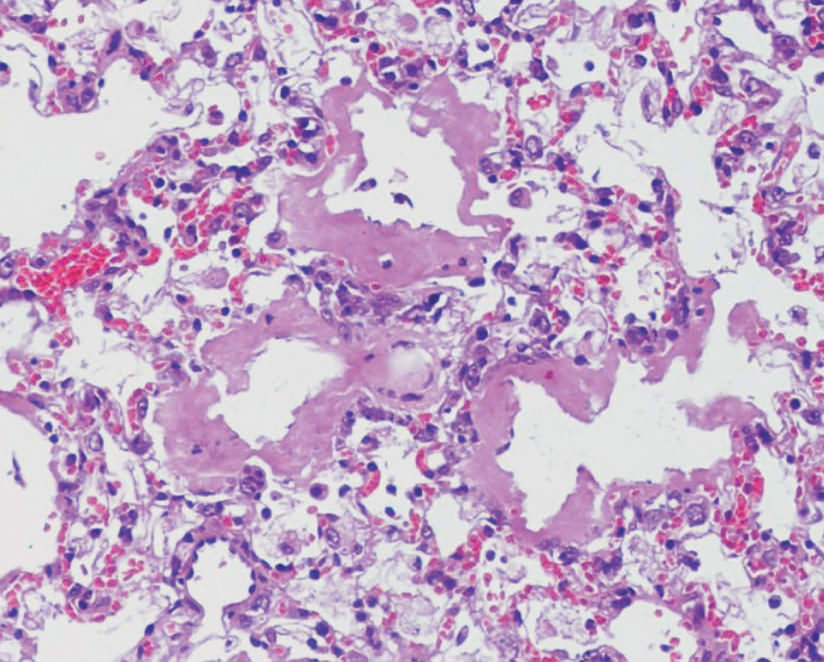
\includegraphics{./images/Image00122.jpg}
 \captionsetup{justification=centering}
 \caption{病毒性肺炎(HE染色,中倍)\\ {\small 肺泡壁充血,巨噬细胞和淋巴细胞浸润,肺泡腔内渗出物形成透明膜}}
\label{fig7-13}
  \end{figure}

\paragraph{临床病理联系}
病毒血症可引起发热及全身中毒症状。由于支气管、细支气管炎症刺激可引起剧烈咳嗽。若肺泡腔内渗出物少,肺部啰音及实变体征不明显。严重病例或继发细菌感染时,肺部出现实变体征,伴有严重的全身中毒和缺氧症状,甚至导致心、肺功能不全,预后不良。

{【附】SARS}

严重急性呼吸道综合征(severe acute respiratory
syndrome,SARS)是由冠状病毒(SARS病毒)引起的一种新的呼吸系统传染性疾病。中国广东省首先发现,最早的病例出现在2002年11月中旬。目前已有多个国家报告发现了SARS病例。本病主要通过近距离空气飞沫和密切接触传播,临床主要表现为肺炎,有比较强的传染力。人群普遍易感,医护人员是本病的高危人群。潜伏期为2~12天,通常为4~5天。传染性主要在急性期(发病早期),尤以刚发病时最强。当病人被隔离及采取抗病毒、提高机体免疫力等治疗措施后,机体开始识别病毒并出现针对SARS的特异性免疫反应来抵抗和中和病毒。随着疾病的康复,SARS病毒逐渐被机体所清除,其传染性也随之消失。SARS起病急,以发热为首发症状,体温一般超过38℃,偶有畏寒;可伴有头痛、关节酸痛、肌肉酸痛、乏力、腹泻;常无上呼吸道其他症状;可有咳嗽,多为干咳、少痰,偶有血丝痰;可有胸闷,严重者出现呼吸加速,气促,或明显呼吸窘迫。肺部体征不明显,部分病人可闻少许湿啰音,或有肺实变体征。实验室检查发现:外周血白细胞计数一般不升高,或降低;常有淋巴细胞计数减少。胸部X线检查为肺部有不同程度的片状、斑片状浸润性阴影或呈网状改变,部分病人进展迅速,呈大片状阴影,常为双侧改变,阴影吸收消散较慢。肺部阴影与症状体征可不一致等。

一、病理变化

SARS死亡病例尸检显示该病以肺和免疫系统的病变最为突出,心、肝、肾、肾上腺等实质性器官也不同程度受累。

1.
肺部病变 肉眼观:双肺呈斑块状实变,严重者双肺完全性实变;表面暗红色,切面可见肺出血灶及出血性梗死灶。镜下观:以弥漫性肺泡损伤为主,肺组织重度充血、出血和肺水肿,肺泡腔内充满大量脱落和增生的肺泡上皮细胞及渗出的单核细胞、淋巴细胞和浆细胞。部分肺泡上皮细胞胞质内可见典型的病毒包涵体,电镜证实为病毒颗粒。肺泡腔内可见广泛透明膜形成,部分病例肺泡腔内渗出物出现机化,呈肾小球样机化性肺炎改变。肺小血管呈血管炎改变,部分管壁可见纤维素样坏死伴血栓形成,微血管内可见纤维索性血栓。

2.
脾和淋巴结病变 脾体积略缩小,质软。镜下见脾小体高度萎缩,脾动脉周围淋巴鞘内淋巴细胞减少,红髓内淋巴细胞稀疏,白髓和被膜下淋巴组织大片灶状出血坏死。肺门淋巴结及腹腔淋巴结固有结构消失,皮髓质分界不清,皮质区淋巴细胞数量明显减少,常见淋巴组织呈灶状坏死。心、肝、肾、肾上腺等器官均有不同程度变性、坏死和出血等改变。

二、结局及并发症

从目前掌握的SARS的传染过程来看,SARS病人的传染性主要在急性期(发病早期),尤以刚发病时为强。随着疾病的康复,SARS病毒逐渐被机体所清除,其传染性也随之消失。所以,SARS病人康复出院后是不会传染他人的。

不足5%的严重病例可因呼吸衰竭而死亡,其并发症及后遗症有待进一步观察确定。

\section{硅肺}

在职业活动中,因长期吸入有害粉尘,引起以肺广泛纤维化为主要病变的疾病,统称尘肺(pneumoconiosis)。尘肺是我国一种法定职业病。硅肺(silicosis)又称矽肺,是尘肺中最常见的类型,也是危害最严重的一种职业病。是人体在生产环境中长期吸入大量含游离二氧化硅(SiO{2}
)粉尘微粒所引起的以肺纤维化为主要病变的全身性疾病。该病发展缓慢,即使在脱离硅尘作业后,病变仍然继续发展。病人多在接触硅尘10~15年后才发病。若因吸入高浓度、高游离二氧化硅含量的硅尘,经1~2年后发病者,称速发型硅肺。硅肺的早期即有肺功能损害,但因肺的代偿能力很强,病人往往无症状;随着病变的发展,尤其是合并肺结核和肺心病时,则逐渐出现不同程度的呼吸和心功能障碍。

\subsection{病因和发病机制}

游离二氧化硅是硅肺的致病因子。硅肺的发生、发展与硅尘中游离二氧化硅的含量,生产环境中硅尘的浓度、分散度,从事硅尘作业的工龄及机体防御功能等因素有关。一般来说,直径大于5
μm的硅尘往往被阻留在上呼吸道,并可被呼吸道的防御装置清除。直径小于5
μm的硅尘才能被吸入肺泡,并进入肺泡间隔,引起病变,其中尤以1~2
μm的硅尘微粒引起的病变最为严重。

吸入肺泡内的硅尘微粒被肺巨噬细胞吞噬,沿肺淋巴流经细支气管周围、小血管周围、小叶间隔和胸膜再到达肺门淋巴结。当淋巴道阻塞后,硅尘沉积于肺间质内引起硅肺病变。若局部沉积的硅尘量多,引起肺巨噬细胞局灶性聚积,可导致硅结节形成;若硅尘散在分布,则引起弥漫性肺间质纤维化。

硅肺的发病机制尚未完全阐明。一般认为,游离二氧化硅颗粒进入肺泡后,被聚集在肺淋巴管起始部位的肺巨噬细胞所吞噬,游离二氧化硅对巨噬细胞有极强的毒性作用,可致其自溶死亡,二氧化硅被吞噬后,被包裹在吞噬细胞溶酶体中,由于石英表面的羟基和巨噬细胞溶酶体膜脂蛋白结构上的氢原子受体(氧、氮及硫原子)间形成氢键,引起细胞膜的改变和通透性的变化,导致巨噬细胞溶酶体崩解,并释放出酸性水解酶进入细胞内,继而导致巨噬细胞死亡,并再次将石英粒子释放,形成恶性循环,造成更多的细胞受损,受损的巨噬细胞释放出非脂类“致纤维化因子”,刺激成纤维细胞,合成胶原纤维增多,形成以胶原纤维为中心的病灶结节-硅结节,硅结节向全肺扩展并相互融合,造成双肺弥漫性损害。纤维化不仅局限于肺内,也存在于巨噬细胞所迁移到的淋巴结内。在许多硅肺病人中已发现血清γ-球蛋白水平增高,自身抗体的存在,以及在硅肺病变中存在γ-球蛋白,故认为硅肺发生与免疫发病有关。

\subsection{病理变化}

硅肺的基本病理变化是肺组织内硅结节形成和弥漫性间质纤维化。硅结节是硅肺的特征性病变,结节境界清楚,直径2~5
mm,呈圆形或椭圆形,灰白色,质硬,触之有砂样感。随着病变的发展,结节可融合成团块状,在团块的中央,由于缺血、缺氧而发生坏死、液化,形成硅肺性空洞。硅结节的形成过程大致分为三个阶段:①细胞性结节,由吞噬硅尘的巨噬细胞局灶性聚积而成,巨噬细胞间有网状纤维,这是早期的硅结节(图\ref{fig7-14}A);②纤维性结节,由成纤维细胞、纤维细胞和胶原纤维构成(图\ref{fig7-14}B);③玻璃样结节,玻璃样变从结节中央开始,逐渐向周围发展,往往在发生玻璃样变的结节周围又有新的纤维组织包绕。

镜下,典型的硅结节是由呈同心圆状或旋涡状排列的、已发生玻璃样变的胶原纤维构成。结节中央往往可见内膜增厚的血管。用偏光显微镜观察,可以发现沉积在硅结节和肺组织内呈双屈光性的硅尘微粒。除硅结节外,肺内还有不同程度的弥漫性间质纤维化,范围可达全肺2/3以上。此外,胸膜也因纤维组织弥漫增生而广泛增厚,甚至可厚达1~2
cm。肺门淋巴结内也有硅结节形成和弥漫性纤维化及钙化,淋巴结因而肿大、变硬。

\begin{figure}[!htbp]
 \centering
 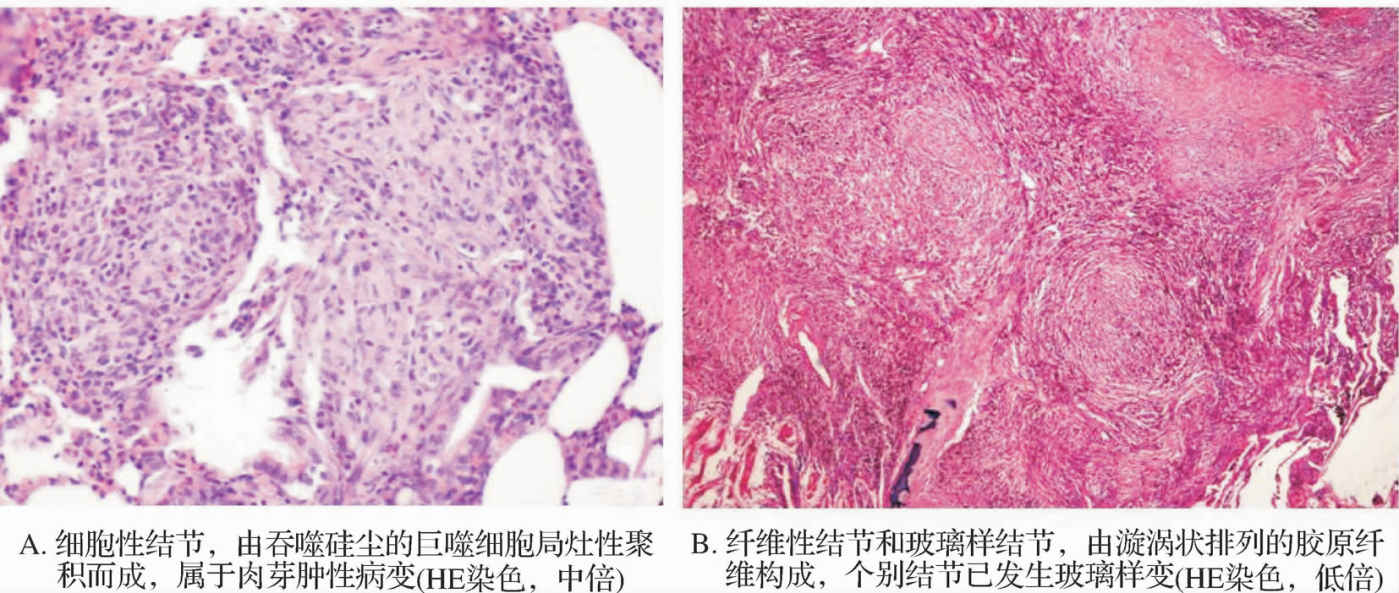
\includegraphics{./images/Image00123.jpg}
 \captionsetup{justification=centering}
 \caption{硅结节}
 \label{fig7-14}
  \end{figure} 

\subsection{硅肺的分期}

根据肺内硅结节的数量、分布范围和直径大小,可将硅肺分为三期。

Ⅰ期硅肺:硅结节主要局限在淋巴系统。肺组织中硅结节数量较少,直径一般在1~3
mm,主要分布在两肺中、下叶近肺门处。X线检查,肺野内可见一定数量的类圆形或不规则小阴影,其分布范围不少于两个肺区。此时,肺的重量、体积和硬度无明显改变。胸膜上可有硅结节形成,但胸膜增厚不明显。

Ⅱ期硅肺:硅结节数量增多、体积增大,可散于全肺,但仍以肺门周围中、下肺叶较密集,总的病变范围不超过全肺;X线表现为肺野内有较多量直径不超过1
cm的小阴影,分布范围不少于四个肺区。此时,肺的重量、体积和硬度均有增加,胸膜也增厚。

Ⅲ期硅肺:硅结节密集融合成块。X线表现有大阴影出现,其长径不小于2
cm,宽径不小于7
cm。此时,肺的重量和硬度明显增加。解剖取出新鲜肺标本可竖立不倒,切开时阻力甚大,并有砂粒感。浮沉试验,全肺入水下沉。团块状结节的中央可有硅肺空洞形成。结节之间的肺组织常有明显的灶周肺气肿,有时肺表面还可见到肺大泡。

\subsection{硅肺的常见并发症}

\paragraph{硅肺结核病}
硅肺合并结核病时称为硅肺结核病。Ⅲ期硅肺的合并率达60%~70%。硅肺病人易合并肺结核可能是因游离二氧化硅对巨噬细胞的毒性损害以及肺间质弥漫性纤维化,导致肺的血液循环和淋巴循环障碍,从而降低了肺组织对结核杆菌的防御能力的缘故。硅肺结核病时,硅肺病变和结核病变可分开存在,也可混合存在。硅肺结核病的病变比单纯硅肺和单纯肺结核的病变发展更快,累及范围更广,更易形成空洞。硅肺结核性空洞的特点是数目多、直径大、空洞壁极不规则。较大的血管易被侵蚀,可导致病人大咯血死亡。

\paragraph{肺感染}
由于硅肺病人抵抗力低,又有慢性阻塞性肺疾病,小气道引流不畅,故易继发细菌或病毒感染。尤其在有弥漫性肺气肿的情况下,肺感染可诱发呼吸衰竭而致死。

\paragraph{慢性肺源性心脏病}
有60%~75%的硅肺病人并发肺心病。这是因为肺间质弥漫性纤维化,肺毛细血管床减少,肺循环阻力增加。同时,硅结节内小血管常因闭塞性血管内膜炎,管壁纤维化,使管腔狭窄乃至闭塞,血管也扭曲、变形,尤以肺小动脉的损害更为明显,加之因呼吸功能障碍造成的缺氧,引起肺小动脉痉挛,均可导致肺循环阻力增加、肺动脉高压和右心室肌壁肥厚,心腔扩张。重症病人可因右心衰竭而死亡。

\paragraph{肺气肿和自发性}
气胸晚期硅肺病人常有不同程度的弥漫性肺气肿,主要是阻塞性肺气肿,有时在脏层胸膜下还可出现肺大泡。气肿囊腔破裂引起自发性气胸。

\section{呼吸系统常见恶性肿瘤}

\subsection{鼻咽癌}

鼻咽癌(nasopharyngeal
carcinoma,NPC)是发生于鼻咽部上皮组织的恶性肿瘤,在我国较为常见。尤其多见于广东、广西、福建等南方地区,有明显的地区多发性。男性患者为女性的2倍,患者多在40~50岁。

\subsubsection{病因及发病机制}

鼻咽癌的病因迄今尚未完全阐明,可能与以下因素相关。

\paragraph{EB病毒}
资料显示100%鼻咽癌患者中有EB病毒的基因组,癌细胞内存在EBV-DNA及EB核抗原(EBNA),患者血清内还有高效价的抗EB病毒抗体,但EB是鼻咽癌的致病启动因素还是其他致癌物质的辅助作用因素尚需进一步研究。

\paragraph{环境致癌物质}
某些环境化学致癌物如亚硝胺、多环芳烃类化合物、微量元素镍等可能与鼻咽癌的发生有关。

\paragraph{遗传因素}
鼻咽癌发病有明显的地区性差异,高发区居民移居他地或国外,其后裔的发病率仍远远高于当地居民。部分鼻咽癌患者还有家族发病倾向,因此在其发病中可能有遗传性易感因素。

\subsubsection{病理变化}

鼻咽癌最常发生于鼻咽顶部,其次为侧壁及咽隐窝。有时还可同时在顶部及侧壁发生。

肉眼观:鼻咽癌呈结节型、菜花型、浸润型及溃疡型四种形态,其中以结节型最常见。早期局部黏膜仅显粗糙、增厚或稍稍隆起,临床检查时易被忽略。有时原发部位未发现肿瘤时已发生颈部淋巴结转移。

绝大多数鼻咽癌起源于鼻咽黏膜柱状上皮的储备细胞,该细胞是一种原始多能性的细胞,既可向柱状上皮方向分化,又可向鳞状上皮方向分化。因此,鼻咽癌的组织学分类较为复杂,迄今还没有统一的鼻咽癌病理学分类。一般来说,可分为两类。

\paragraph{鳞状细胞癌}
按细胞分化程度,可分为角化型和非角化型。

角化型鳞状细胞癌极少见,主要发生于老年患者,此型较少见,一般认为其发生与EB病毒无关。非角化型鳞状细胞癌最为多见,癌细胞呈多角形、卵圆形或梭形,无细胞角化现象,其发生与EB病毒感染关系密切。非角化型癌还可进一步分为分化型和未分化型。分化型即低分化鳞状细胞癌。未分化型又可分为分化极差的鳞状细胞癌和泡状核细胞癌。

\paragraph{腺癌}
高分化腺癌少见,癌细胞排列成腺泡状或管状。低分化腺癌癌细胞呈不规则条索状或片状排列,有时可见到腺腔结构或围成腺腔的倾向。

在鼻咽癌的组织学分型中,非角化型鳞状细胞癌最为常见,其次为未分化型的泡状核细胞癌。低分化腺癌较少,高分化鳞状细胞癌及腺癌最少。

\subsubsection{扩散及转移}

\paragraph{直接蔓延}
鼻咽部解剖解构复杂,肿瘤向上可侵犯颅内,向下扩展到达口咽,向下后方则侵犯梨状隐窝、会厌及喉腔上部,向外侧扩展可侵犯耳咽管至中耳,向后扩展则穿过鼻咽后壁侵犯上段颈椎,向前扩展则进入鼻腔甚至侵入眼眶。

\paragraph{淋巴道转移}
鼻咽黏膜固有层有丰富的淋巴管,故本癌可早期经淋巴道转移。颈淋巴结转移常为同侧,其次为双侧,极少只呈对侧转移。

\paragraph{血道转移}
常转移至肝、肺、骨,其次是肾、肾上腺及胰腺等处。

\subsubsection{临床病理联系}

鼻咽癌临床表现多样,常有鼻衄、鼻塞、耳鸣、听力减退、颈部肿块、复视及偏头痛等症状。当症状明显时多已进入进展期或晚期,治愈率极低,故早期诊断极为重要。

\begin{framed}
{案例7-1}

{【病例摘要】}

患者,男,65岁,因咳嗽、咳痰、痰中带血3个月入院。患者三月前开始出现刺激性咳嗽,自服止咳药未好转,痰中可出现血丝,近一月来症状加重。自发病以来患者体重下降8
kg。既往40余年吸烟史,平均每日1.5包,无酗酒史。入院后体检呈消瘦貌,神萎,血常规示中度贫血。胸片示肺门处一3cm×4cm占位影,怀疑支气管肺癌。

{【问题】}

(1)该患者怀疑支气管肺癌的依据为哪些?

(2)后行支气管镜检查,确诊为小细胞肺癌,试描述肿瘤镜下的组织学特征。
\end{framed}

\subsection{肺癌}

肺癌(lung
carcinoma)又称支气管肺癌,是最常见的恶性肿瘤之一。每年全世界有超过130万人被确诊患有肺癌,超过110万人死于肺癌。我国肺癌的发病率在20世纪70年代至90年代上升一倍多之后,近10年里继续呈明显上升趋势,目前肺癌已成为我国危害最大的癌症。肺癌多发生于45岁以上的中老年人,在55~75岁患病率最高,男女性别比例为2∶1。近年来,由于女性吸烟者的不断增加,女性比例相应上升。

\subsubsection{病因与发病机制}

肺癌的病因较复杂,其发生与下列因素有关。

\paragraph{吸烟}
吸烟是肺癌发生的重要危险因素,大约有3/4的肺癌患者有重度吸烟史。吸纸烟者肺癌的死亡率比不吸烟者高10~13倍。吸烟的量越多、吸烟的时间越长、开始吸烟的年龄越早,肺癌的死亡率越高。戒烟后则随戒烟时间的延长,肺癌发生率逐渐降低。卷烟燃烧的烟雾中含有超过1
200种化学物质,其中多环芳烃、3,4-苯并芘、放射性元素及砷等多种物质均具有致癌作用。3,4-苯并芘等多环芳烃碳氢化合物在人体内的芳烃羟化酶(AHH)的作用下转变为环氧化物而成为终致癌物,可导致细胞基因突变。由于不同人体内AHH的酶活性不同,因此吸烟致癌存在着个体差异。

\paragraph{物理化学致癌因子}
目前比较公认的致癌因子有烟草燃烧的产物、石棉、砷、铬、镍、铍、煤焦油、沥青、烟尘、芥子气、二氯甲醚等。如果长期接触这些物质,可以诱发肺癌。我国云南锡矿工人的肺癌发生率高达435.44/10万,井下作业较地面作业工人肺癌发病率高20倍。可能与工作中长期接触化学致癌物质和放射性物质有关。

\paragraph{大气污染}
煤、汽油、柴油等燃烧后的废气或烟尘、行驶机动车的排气均可造成空气污染。被污染的空气中含有3,4-苯并芘、二乙基亚硝胺和砷等致癌物。调查表明,工业发达国家肺癌发病率比工业落后国家高、城市比农村高、大城市比中小城市高。

\paragraph{基因改变}
各种致癌因素可引起细胞的基因变化而导致细胞发生癌变。目前已知在肺癌中有多种癌基因的突变或肿瘤抑制基因的失活,其中KRAS、c-Myc、P53、Rb和bcl-2基因都是研究的热点。有关遗传或基因因素在肺癌发生过程中的作用,有待于进一步研究探索。

\subsubsection{病理变化}

\paragraph{大体类型}
根据肿瘤的发生部位可把肺癌分为三种类型:中央型、周围型和弥漫型,与临床X线的肺癌分型相一致。

(1)中央型:此型最常见,多起源于主支气管或叶支气管等大支气管,肿瘤位于肺门部,常破坏支气管壁向周围肺组织浸润、扩展。晚期形成巨块,常包绕癌变的支气管(图\ref{fig7-15}A)。

(2)周围型:此型发生率仅次于中央型,多起源于肺段以下的末梢支气管或肺泡。常在靠近胸膜的肺周边部形成孤立的癌结节。肉眼形态多为结节型(图\ref{fig7-15}B)。

(3)弥漫型:此型少见。肉眼观察:多数呈播散性的粟粒性结节,弥漫侵犯部分肺大叶或全肺叶,似肺炎或播散性肺结核(图\ref{fig7-15}C)。

\begin{figure}[!htbp]
 \centering
 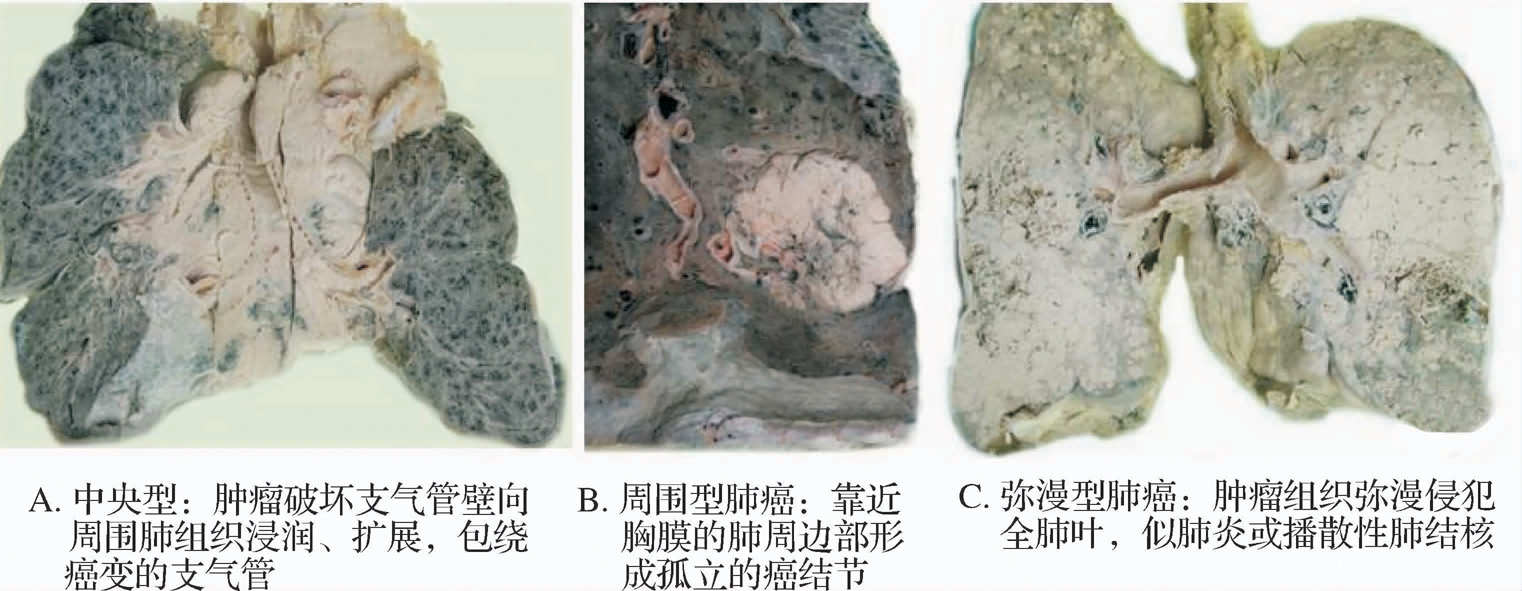
\includegraphics{./images/Image00124.jpg}
 \captionsetup{justification=centering}
 \caption{肺癌大体形态}
 \label{fig7-15}
  \end{figure} 

\paragraph{组织学类型}
世界卫生组织(WHO)最新分类中把肺癌分为鳞状细胞癌、腺癌、大细胞癌、腺鳞癌、神经内分泌癌、肉瘤样癌、其他类型癌和唾液腺来源的癌等8种类型。不同组织学类型在临床表现、治疗手段的选择及预后上均不相同。

(1)鳞状细胞癌:是肺癌最常见类型之一,绝大多数为中老年患者,多有吸烟史。多来自段以上或主支气管,肉眼属中央型,纤支镜检查易被发现,痰脱落细胞学检查阳性率高。高分化鳞癌多有角化珠形成,低分化鳞癌仅有少量细胞角化。

(2)腺癌:也是原发性肺癌中最常见类型之一,且近年来发病率有不断上升的趋势。肺腺癌多数为周围型,女性患者较多,患者不吸烟但多有被动吸烟史。腺癌常位于肺周边部呈孤立结节,边界清楚,常累及胸膜。高分化癌可见癌组织形成腺管或乳头,并有黏液分泌。

(3)神经内分泌细胞癌:主要包含小细胞癌、大细胞神经内分泌癌和类癌。小细胞癌为仅低于肺鳞癌及腺癌的相对常见的一型肺癌。其发生率占原发性肺癌的15%~20%。发病年龄较鳞癌低,好发于中年男性,与吸烟及职业性接触有一定关系。肿瘤恶性度极高,生长迅速。多有早期转移,一般不适合手术切除,但对化疗及放疗敏感。本型癌细胞小呈短梭形(燕麦型,图\ref{fig7-16})或小圆形(淋巴细胞样),核浓染,胞浆稀少形似裸核。癌细胞常密集成群,有时围绕小血管排列成假菊形团样结构。电镜下可见一部分癌细胞胞浆含有神经分泌颗粒,现认为该肿瘤起源于APUD系统,可伴有异位内分泌综合征。

\begin{figure}[!htbp]
 \centering
 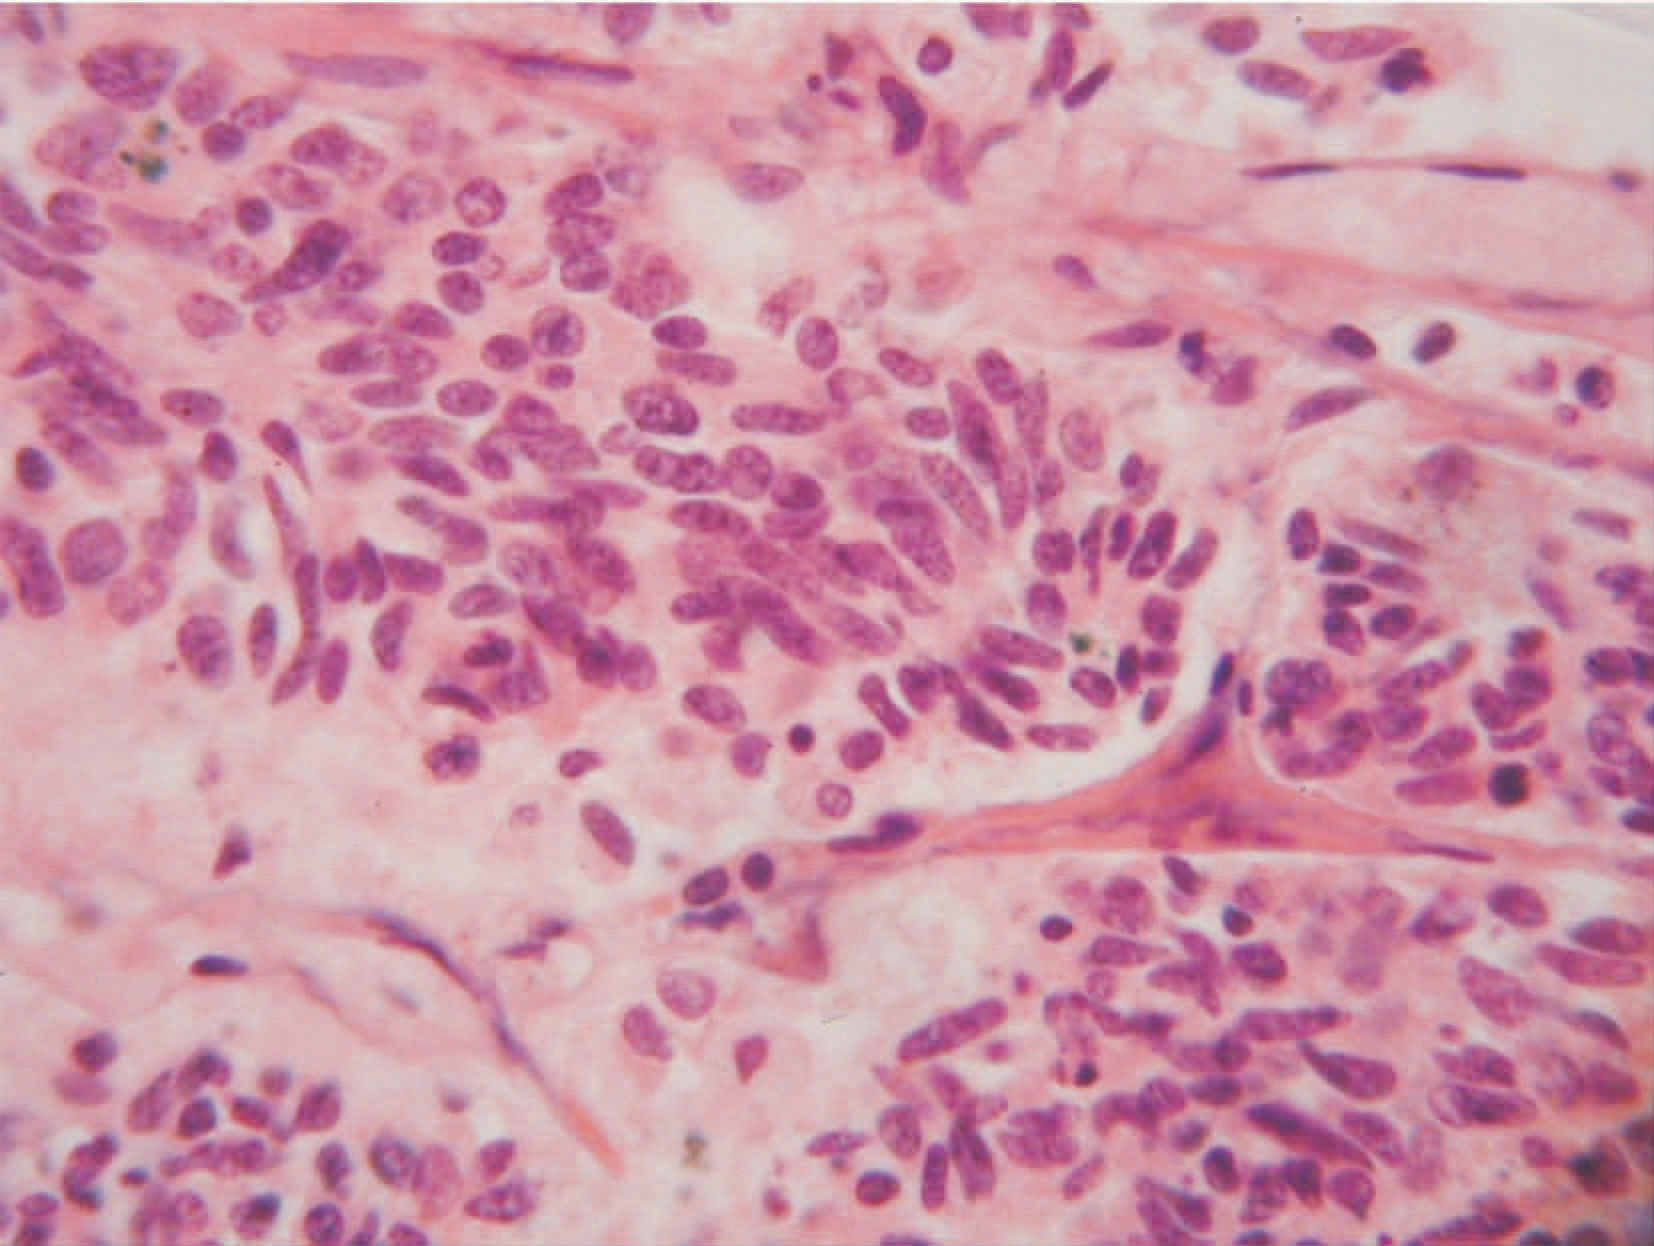
\includegraphics{./images/Image00125.jpg}
 \captionsetup{justification=centering}
 \caption{燕麦细胞癌(HE染色,高倍)\\ {\small 癌细胞小呈短梭形或小圆形,常密集成群,围绕小血管排列成假菊形团样结构}}
\label{fig7-16}
  \end{figure}

(4)大细胞癌:肺大细胞癌属于未分化癌,恶性度高,癌生长迅速,早期发生转移。

(5)腺鳞癌:此型肺癌含有腺癌细胞及鳞癌细胞两种成分,属于混合性癌。现认为此型肺癌发生自支气管上皮的具多向分化潜能的干细胞。

(6)肉瘤样癌:为近年WHO新列出的一种肺癌分类,癌分化不成熟,恶性度高,有多形性、梭形细胞性、巨细胞癌及癌肉瘤等多种亚型。

\subsubsection{扩散与转移}

\paragraph{直接蔓延}
中央型肺癌常直接侵及肿瘤周围组织如纵隔、心包及周围血管,或沿支气管向同侧甚至对侧肺组织蔓延。周围型肺癌可直接侵犯胸膜,在胸壁生长。

\paragraph{转移}
肺癌沿淋巴道转移时首先转移至肺门淋巴结,再扩散至纵隔、锁骨上、腋窝和颈部淋巴结。周围型肺癌的癌细胞可到达胸膜下淋巴丛,引起胸膜腔的血性渗出液。血行转移常见于肝、脑、肾上腺、骨及肾等处。

\subsubsection{临床病理联系}

肺癌早期因症状不明显易被忽视。患者可有咳嗽、痰中带血丝及胸痛等症状。肿瘤压迫或阻塞支气管可引起远端肺组织的化脓性炎、脓肿形成。癌组织侵及胸膜引起癌性胸膜炎、积液。侵犯纵隔内压迫上腔静脉引起面颈部水肿及颈、胸部静脉曲张(上腔静脉综合征)。肺尖部肺癌易侵犯交感神经引起病侧眼睑下垂、瞳孔缩小和胸壁皮肤无汗等交感神经麻痹综合征(Horner综合征)。有异位内分泌作用的肺癌,尤其是小细胞肺癌可因5-羟色胺分泌过多而引起类癌综合征,表现为支气管哮喘、心动过速、水样腹泻和皮肤潮红等。

\begin{center}
    \textbf{知识链接}
\end{center}
\chapterabstract{肺癌生物治疗是一种利用细胞生物学与分子生物学手段调节机体免疫系统功能或肿瘤生长,从而达到抑瘤目的的治疗方法,是继手术、放疗、化疗模式之后新兴的治疗手段,它具有常规治疗方法无可比拟的优势,并显示出良好的临床应用前景。具体治疗包括树突状细胞疫苗、相关肿瘤抗原疫苗、肿瘤细胞疫苗、过继性细胞免疫治疗和分子靶向治疗等。肺癌的生物治疗不仅开辟了肺癌全新治疗模式,同时也丰富了肿瘤生物治疗范围。}

\section*{复习与思考}

{一、名词解释}

COPD慢性阻塞性肺气肿 小叶中央型肺气肿 全小叶型肺气肿 肺心病 大叶性肺炎 小叶性肺炎 肺肉质变 硅结节 燕麦细胞癌

{二、问答题}

1. 试述慢性支气管炎的病变特点。

2. 试述支气管扩张症的发病机制。

3. 试述慢性肺源性心脏病的病变及临床病理联系。

4. 试述大叶性、小叶性、间质性肺炎的病变特点及大、小叶性肺炎的鉴别点。

5. 硅肺的病理特点是什么?硅结节是如何形成的?

6. 鼻咽癌的主要组织学类型及其扩散途径是什么?

7. 肺癌的常见病理类型有哪些?

8. 右肺上叶有一直径约1.5
cm的球形病灶,试考虑有哪些病变的可能及其病理特点。

{三、临床病理分析}

病史:患者男性,64岁。慢性咳嗽、咳痰28年,痰通常为白色泡沫样,有时发热伴脓痰。近五年来爬坡即感气急,近两年来稍活动即感气急,时有心悸,面部与下肢水肿。入院前一周开始发热,近三日来高达39℃,气急加重,指唇出现青紫,下肢水肿。

既往史:吸烟30年,日吸一包以上。

体检:体温38.6℃,脉搏100次/分,呼吸24次/分,血压正常,神志清但迟钝。口唇轻度青紫,下肢轻度水肿,颈静脉稍充盈,胸廓呈桶状。腹部略膨胀,肝剑突下二横指,质中,轻度压痛。扣诊,心界扣不出。听诊:两肺可闻及广泛湿啰音,肺动脉瓣第二音亢进。X线胸片,两肺透明度增高,肺纹理增强,两肺下叶有小片状模糊炎性阴影,横膈低平,心影扩大,肺动脉圆锥突起。

讨论题:

1. 试分析患者可能发生的疾病。

2. 试叙述疾病的发生发展过程。

3. 试阐明疾病的病理变化。